\chapter{Implementierung} \label{chapter:implementation}

In diesem Kapitel wird die Implementierung des Backends, Frontends und
Dashboards des Systems beschrieben. Die Implementierung basiert auf der in
\autoref{chapter:conception} erarbeiteten Konzeption.  Zunächst wird die
Umsetzung des Backends beschrieben, welches sämtliche Daten des Systems
speichert und die Speicherung und Manipulation dieser durch entsprechende
Schnittstellen ermöglicht. Hiernach wird die Realisierung des Frontends
entsprechend dem konzipierten Prototypen (vgl. \autoref{sec:interface-design})
beschrieben. Abschließend wird die Implementierung des Dashboards erläutert.

\section{Implementierung des Backends}

In diesem Abschnitt werden die Struktur des Backends und die Implementierung
seiner Funktionalitäten näher erläutert. Die zu implementierenden
Funktionalitäten sind aus \autoref{sec:concept-func} zu entnehmen. Zunächst wird
der Aufbau einer Strapi-Anwendung erläutert und wie diese um die benötigten
Kern-Funktionalitäten erweitert wurde. Anschließend wird die Einbindung von
Push-Benachrichtigungen näher beschrieben. Abschließend wird erklärt, wie die
Feedback-Funktionalität aufbauend auf Push-Benachrichtig\-ung\-en implementiert
wurde.

\subsection{Struktur eines Strapi-Projekts} \label{ssec:impl-backend-structure}

Im Folgenden wird die Struktur des Backends und seiner verschiedenen
Teilkomponenten erläutert. Die Verzeichnisstruktur wird in
\autoref{fig:impl-backend-structure} aufgezeigt. Zur besseren Lesbarkeit werden
einige Dateien und Unterverzeichnisse ausgeblendet. Das Strapi Projekt teilt
sich in vier wesentliche Teilbereiche auf: \textit{API}, \textit{Komponenten},
\textit{Konfiguration} und \textit{Plugins}. Diese vier Teilbereiche finden sich
in der Verzeichnisstruktur in den entsprechenden Ordnern wieder.

\begin{figure}[htpb]
    \centering
    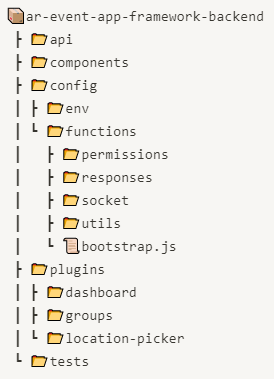
\includegraphics[width=.45\linewidth]{impl/dir_tree_backend.png}
    \caption{Verzeichnisstruktur des Backends}
    \label{fig:impl-backend-structure}
\end{figure}

Der \lstinline[style=code, style=inline]{/api} Ordner beinhaltet die
verschiedenen angelegten APIs des Strapi Projekts. Die meisten der APIs nutzen
hierbei Inhaltstypen (Content-Types). Inhaltstypen werden in Strapi genutzt, um
die Struktur und Art eines Inhalts zu definieren. Die Datenstruktur eines
Inhaltstyps wird dabei durch Attribute festgelegt, welche aus Name, Art und
einstellbaren Einschränkungen bestehen. Strapi stellt drei Arten von
Inhaltstypen bereit: \textit{Kollektionen}, \textit{Einzeltypen} und
\textit{Komponenten}. Während Kollektionen eine Vielzahl von Einträgen
beinhalten können, bestehen Einzeltypen aus nur einem Eintrag. Komponenten sind
hingegen ein wiederverwendbarer Inhaltstyp, welcher nur in Verbindung mit
Kollektionen oder Einzeltypen genutzt werden kann. Sie sind im
\lstinline[style=code, style=inline]{/components} Verzeichnis wiederzufinden.
Die APIs des Systems sind in \autoref{fig:impl-backend-apis} zu sehen.

\begin{figure}[htpb]
    \centering
    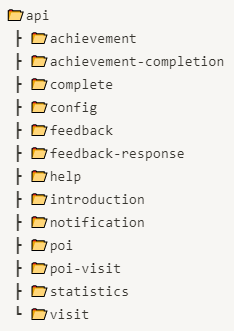
\includegraphics[width=.4\linewidth]{impl/dir_apis.png}
    \caption{Verzeichnisstruktur der Inhaltstypen}
    \label{fig:impl-backend-apis}
\end{figure}

Jede API wird wie folgt unterteilt (\autoref{fig:impl-backend-content-type}
zur Verzeichnisstruktur) und anschließend näher erläutert:

\begin{enumerate}
    \setlength{\itemsep}{1em}
    \item \textbf{Konfiguration (/config)} \\
          Zuweisung von Routen zu Controller-Funktionen unter Angabe von
          \textit{HTTP-Methode, URL} und \textit{Controller-Funktion}.
    \item \textbf{Controller (/controllers)} \\
          Enthält Funktionen, welche Anfragen, wie in der Konfiguration
          festgelegt, empfangen, verarbeiten und eine Antwort oder einen Fehler
          zurücksenden.
    \item \textbf{Modelle (/models)} \\
          Legt Datenstruktur und Name des Inhaltstypen fest. Die verfügbaren
          Datentypen werden in \autoref{fig:impl-backend-types} aufgelistet.
          Falls die API keinen Inhaltstypen nutzt, wird dieses Verzeichnis nicht
          benötigt.
    \item \textbf{Dienste (/services)} \\
          Beinhaltet Funktionen, welche zur Wiederverwendung in verschiedenen
          Controller-Funktionen gedacht sind. Wird genutzt, um die duplizierten
          Programm-Code zu vermeiden.
\end{enumerate}

\begin{figure}[htpb]
    \centering
    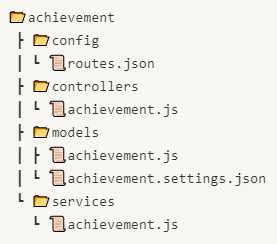
\includegraphics[width=.5\linewidth]{impl/dir_content_type.png}
    \caption{Aufbau eines Inhaltstypen am Beispiel des \textit{Achievement}-Inhaltstypen}
    \label{fig:impl-backend-content-type}
\end{figure}

In der Konfigurationen werden die verschiedenen API Routen des Inhaltstypen
festgelegt. Für jede Route wird die HTTP-Methode, der entsprechende Pfad (z. B.
\textit{/achievements/:id}) und eine Controller-Funktion zugewiesen. Bei der
Wahl der HTTP-Methode ist die Funktion der Route zu beachten und sollte der von
\textcite{RFC7231} beschriebenen Semantik folgen. Beispielsweise sollte eine
Anfrage, welche lediglich Daten zurückerhalten möchte, die \textit{GET}-Methode
nutzen. Eine Anfrage, welche mit übermittelten Daten einen neuen Eintrag im
System erschafft, sollte hingegen die \textit{POST}-Methode nutzen. Alle
voreingestellten Routen sind in \autoref{table:impl-backend-routes} aufgelistet.
Die eingehenden Anfragen werden von der angegebenen Controller-Funktion
verarbeitet. \\
Der Controller besteht aus Funktionen, welche ausgeführt werden, wenn eine für
sie hinterlegte Anfrage erhalten wird. In der Anfrage enthaltene Daten (z. B.
abgeschlossenes Abzeichen) werden an die Funktion übergeben. Innerhalb der
Controller-Funktion wird die Anfrage verarbeitet und eine Antwort
zurückgesendet. Die Antwort können dabei ein beliebiger HTTP-Statuscode, binäre
Daten oder Daten in JSON-Form sein. \\
Das Modell bestimmt die Datenstruktur eines Inhaltstypen und nutzt dabei von
Strapi vorgegebene Datentypen (\autoref{fig:impl-backend-types}). Jeder
Inhaltstyp setzt sich aus ein oder mehreren Attributen zusammen, welche sich aus
einem Namen und einem der Datentypen zusammensetzen. Die Attribute können direkt
in der entsprechenden Datei angelegt oder in der Oberfläche von Strapi
festgelegt werden (\autoref{fig:impl-backend-content-type-builder}).
\\
Dienste werden genutzt, um duplizierten Code zu vermeiden. Logik, welche an
mehreren Stellen benötigt wird, kann in einen Dienst geschrieben werden, um von
dort aus in der API benutzt zu werden. Somit fällt der duplizierte Code weg, was
den Code übersichtlicher und leichter wartbar macht.

\begin{table}[htpb]
    \def\arraystretch{1.25}
    \centering
    \caption{Voreingestellte Routen von Strapi Kollektionen am Beispiel der Abzeichen}
    \label{table:impl-backend-routes}
    \begin{tabular}{lll}
        \uzlhline%
        \uzlemph{Methode} & \uzlemph{Route}              & \uzlemph{Funktion}              \\
        \uzlhline%
        GET               & \textit{/achievements}       & Erhalte alle Abzeichen-Einträge \\
        GET               & \textit{/achievements/:id}   &
        Erhalte Abzeichen-Eintrag mit der angegebenen ID                                   \\
        GET               & \textit{/achievements/count} &
        Erhalte Anzahl der Abzeichen-Einträge                                              \\
        POST              & \textit{/achievements}       &
        Erstellen eines Abzeichen-Eintrags                                                 \\
        DELETE            & \textit{/achievements/:id}   &
        Löschen des Abzeichen-Eintrags mit der angegebenen ID                              \\
        PUT               & \textit{/achievements/:id}   & Verändern des
        Abzeichen-Eintrags mit der angegebenen ID                                          \\
        \uzlhline
    \end{tabular}
\end{table}

\begin{figure}[htpb]
    \centering
    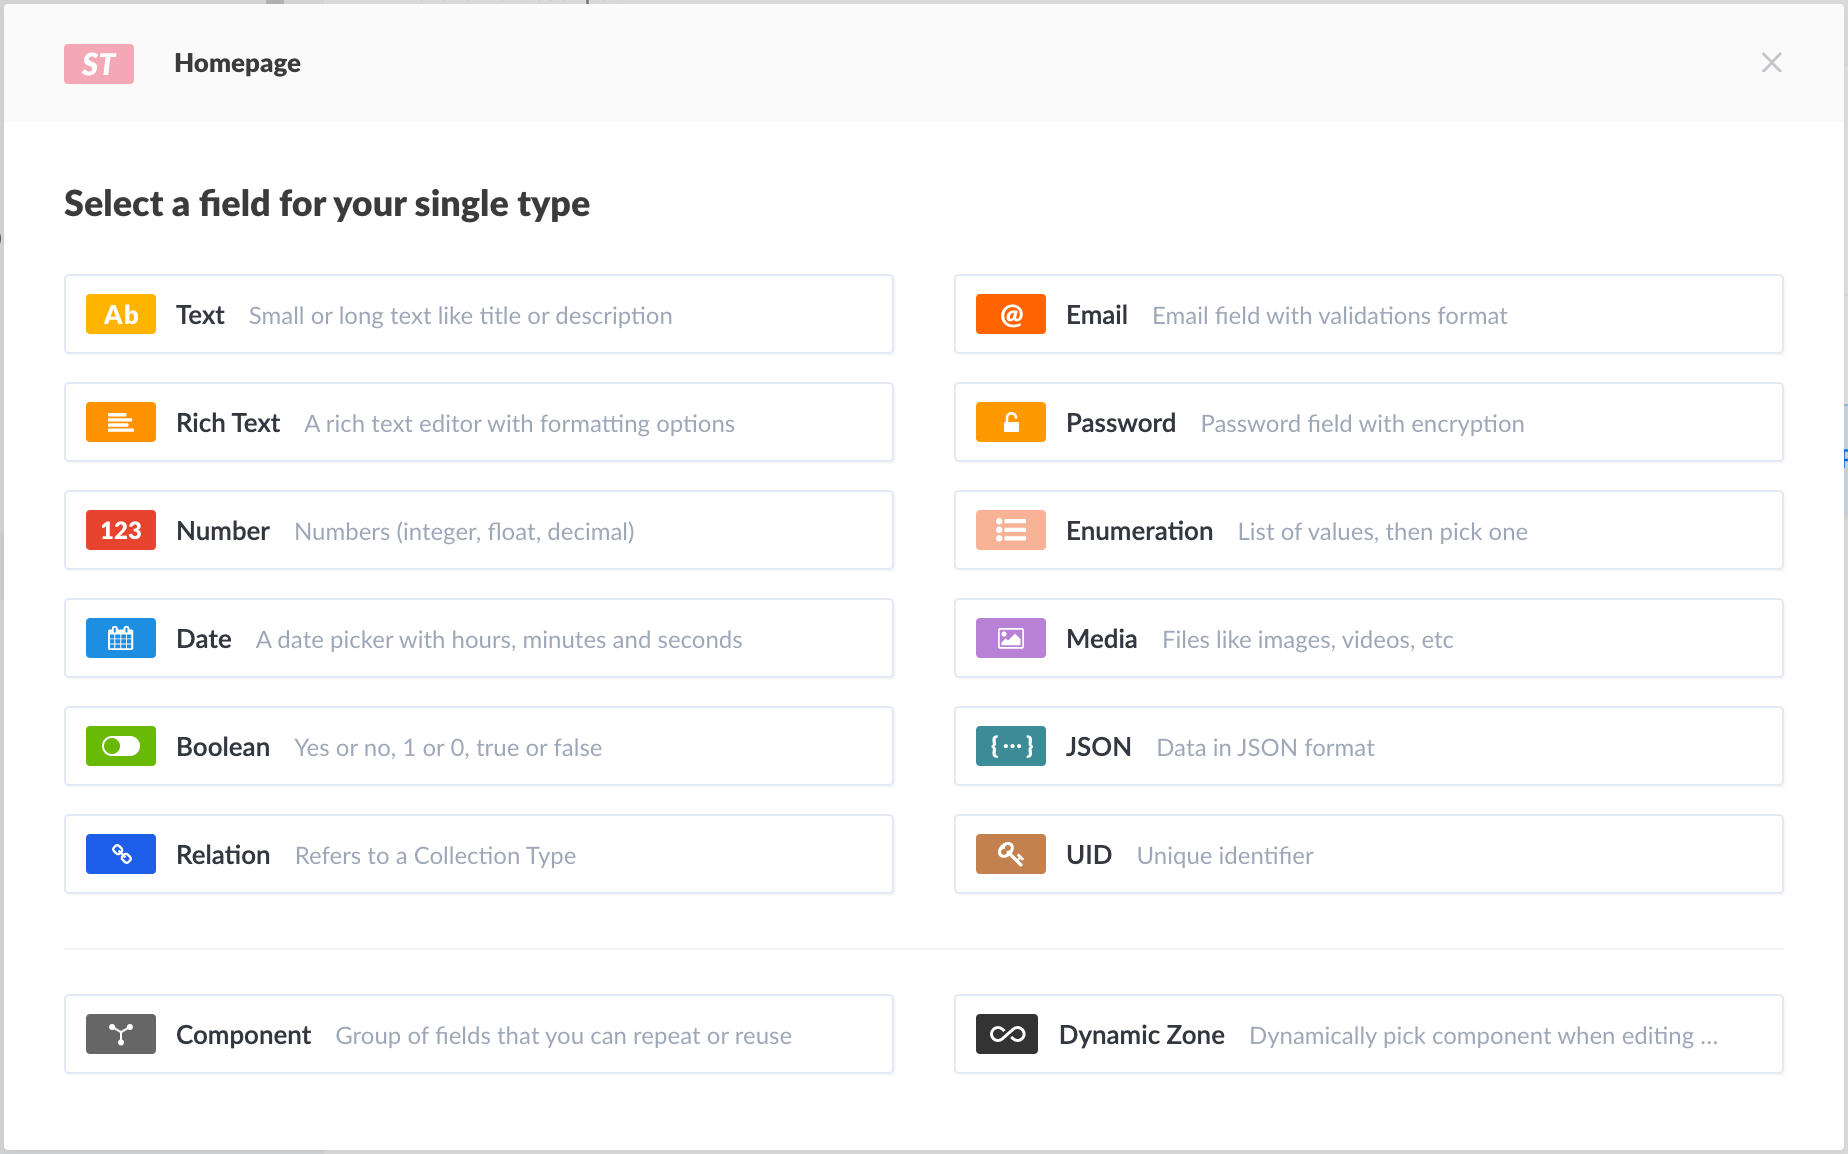
\includegraphics[width=\linewidth]{impl/types.png}
    \caption{Auflistung der verfügbaren Datentypen für Attribute von Inhaltstypen innerhalb Strapis}
    \label{fig:impl-backend-types}
\end{figure}

\begin{figure}[htpb]
    \centering
    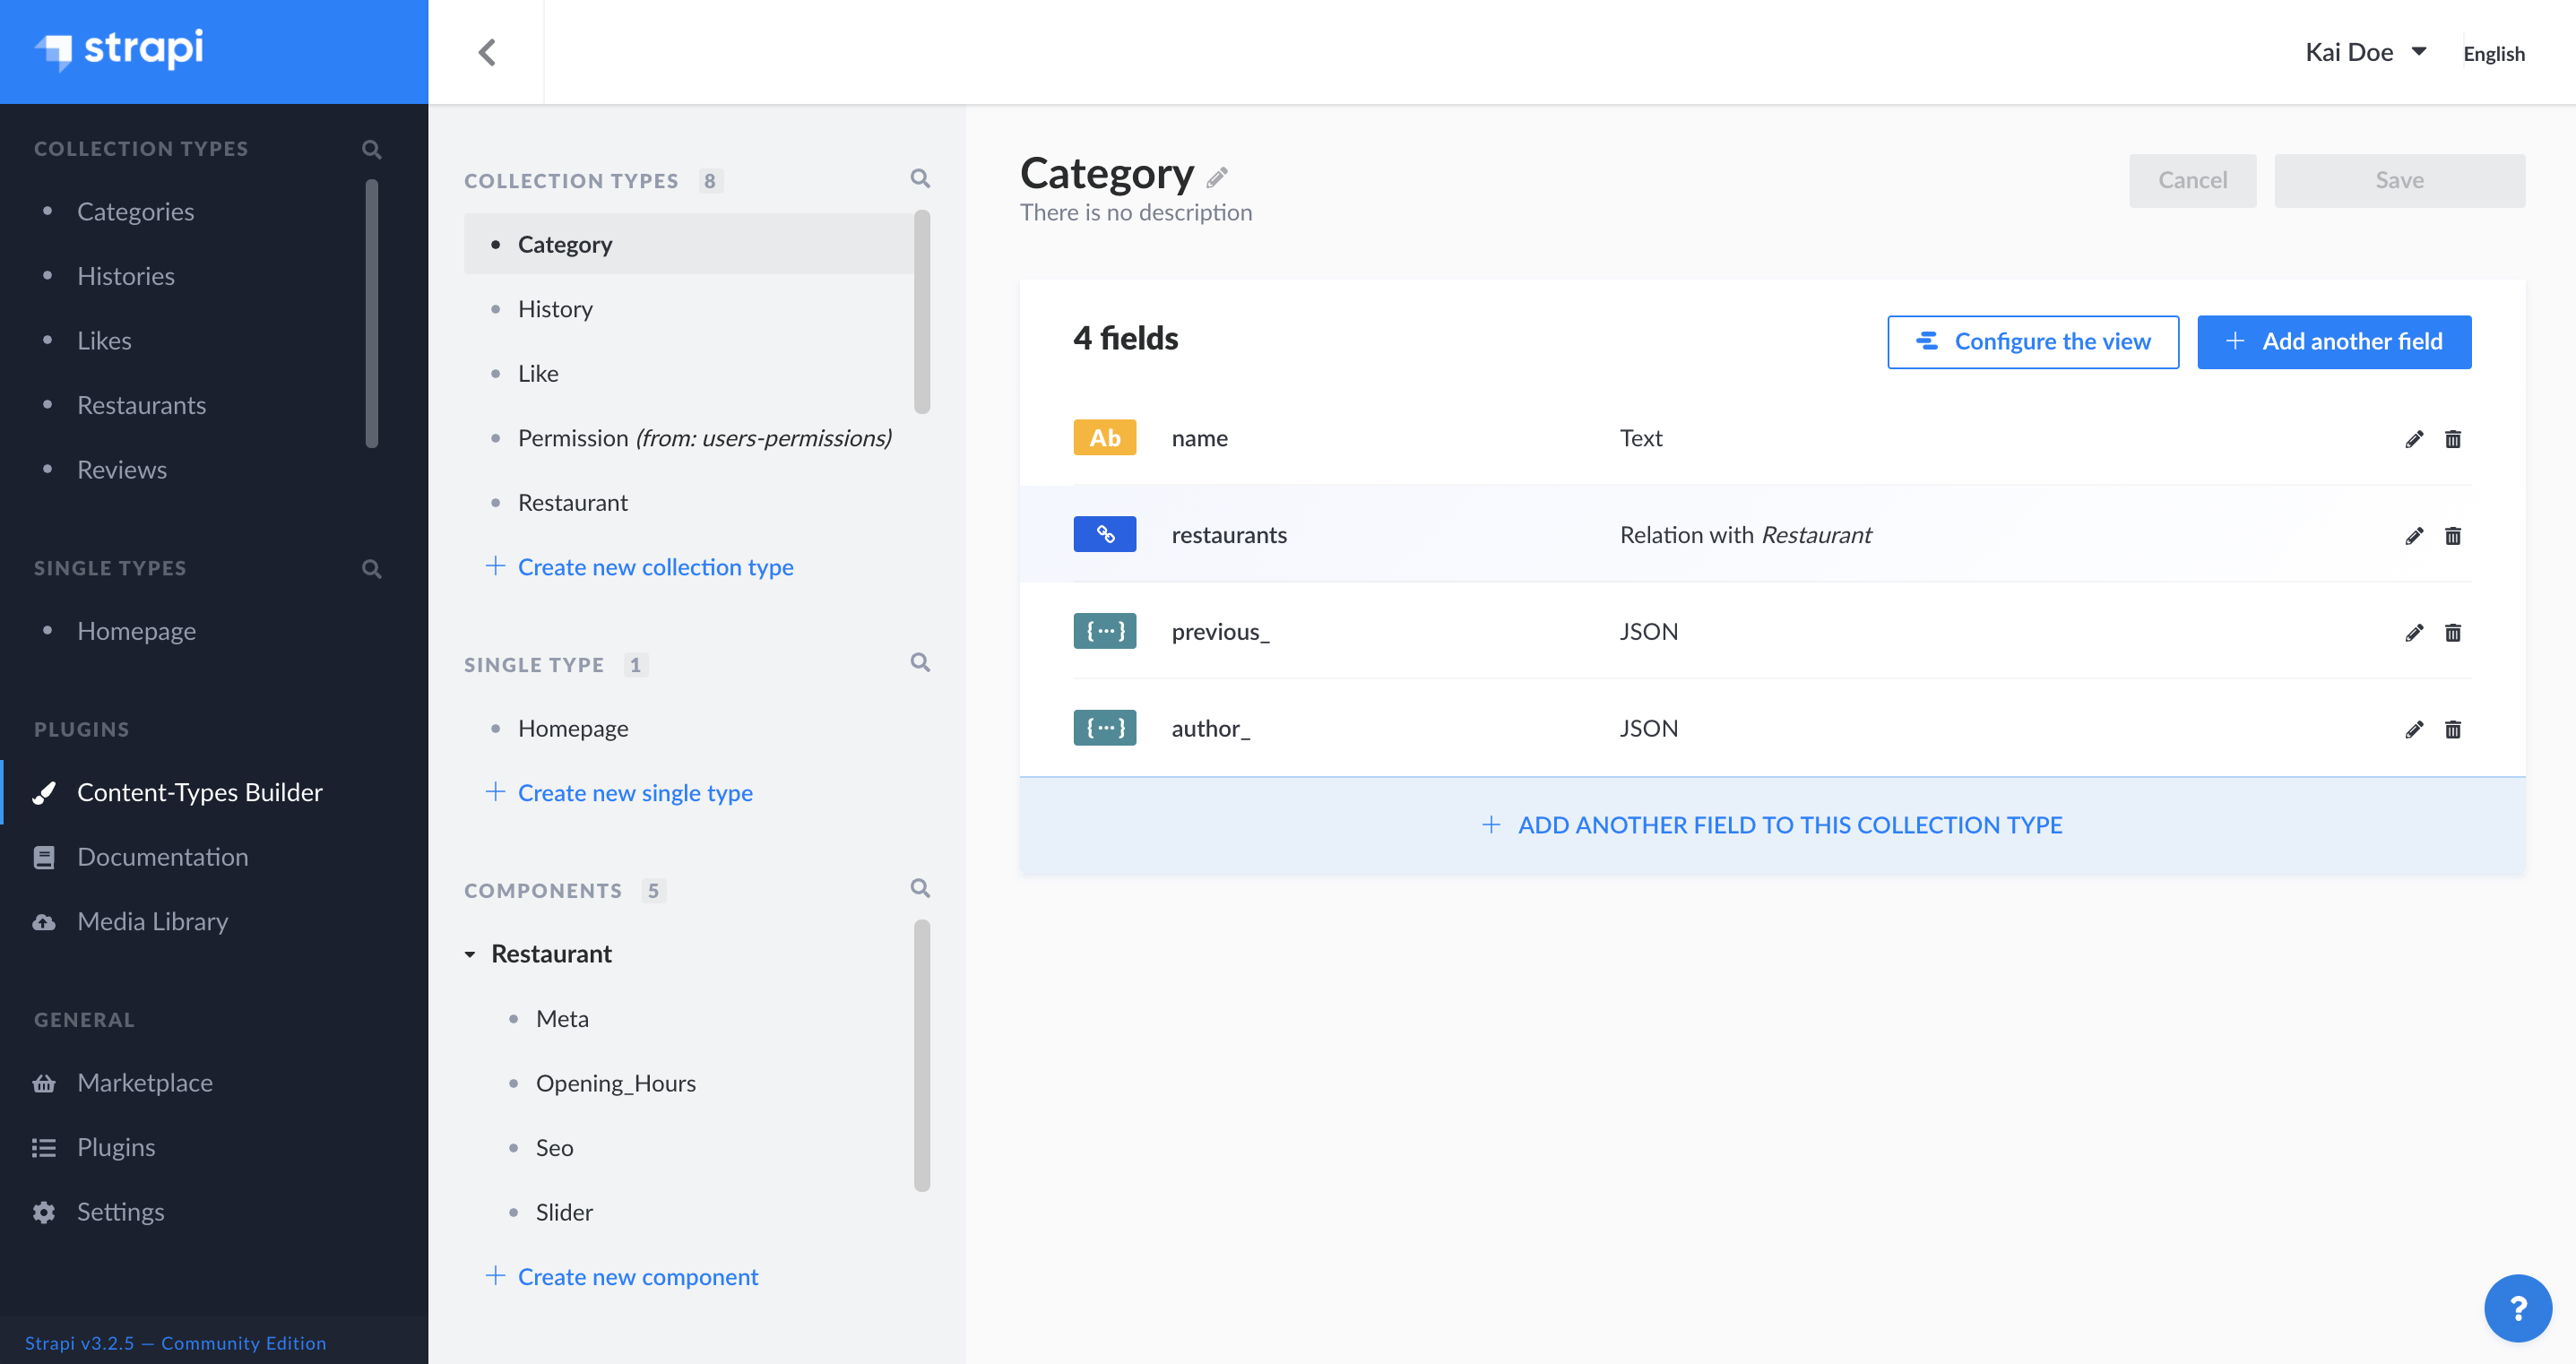
\includegraphics[width=\linewidth]{impl/content-types-builder.png}
    \caption{Oberfläche zum Festlegen der Datenstruktur}
    \label{fig:impl-backend-content-type-builder}
\end{figure}

Das \lstinline[style=code, style=inline]{/config/functions} Verzeichnis des
Projekts enthält Logik, welche zum Start des Systems ausgeführt wird. Die von
der \lstinline[style=code, style=inline]{bootstrap.js} exportierte Funktion
wurde hierbei genutzt, um einen Web-Socket Server zu starten und benötigte
Berechtigungen zu setzen. Auf diese Punkte wird in
\ssecref{ssec:impl-backend-push} genauer eingegangen.

Das \lstinline[style=code, style=inline]{/plugins} Verzeichnis kann genutzt
werden, um Strapi um eigene Module zu erweitern. Möglich ist unter anderem das
Hinzufügen von eigenen Seiten innerhalb der Oberfläche oder die Einbindung einer
eigenen Oberfläche zur Bearbeitung von Attributen. In diesem Projekt sind drei
Plugins zu finden: \textit{groups, dashboard} und \textit{location-picker}. Das
Gruppen-Plugin erfüllt eine Funktion im Backend und wird in
\ssecref{ssec:impl-backend-func} näher erläutert. Das Dash\-board und
Location-Picker-Plugin hingegen werden in \autoref{sec:impl-dashboard}
beschrieben.

Abschließend befinden sich im \lstinline[style=code, style=inline]{/tests}
Verzeichnis Softwaretests, welche genutzt werden, um die korrekte Funktionsweise
der Funktionalitäten, wie in \autoref{sec:concept-func} spezifiziert,
sicherzustellen. Diese sind im Veranstaltungskontext besonders wichtig, da
Fehler während der Veranstaltung im schlimmsten Fall eine komplette
Unterbrechung bedeuten könnten (\anfref{Q30}).

\subsection{Implementierung der Kern-Funktionalitäten} \label{ssec:impl-backend-func}

Nachfolgend wird die Implementierung der Kern-Funktionalitäten des Backends
erläutert, welche aus den Anforderungen aus \autoref{sec:analysis-anf} entnommen
werden. Konkret werden im Folgenden die Implementierung der Stationsbesuche,
Abzeichen und Gruppen beschrieben.

Das Besuchen von Stationen erfolgt mithilfe der Übermittlung des Stations-Codes,
welcher aus vier Zeichen, begrenzt auf Zahlen und großen Buchstaben, besteht.
Der Stations-Code ist unabhängig von der ID der Station und kann manuell
festgelegt werden. Dieses Vorgehen ist nötig, da die inkrementellen IDs der
Stations-Kollektion zu einfach zu erraten wären. Zudem können Stations-Codes so
im Nachhinein angepasst werden, sollte z. B. ein Fehler im Druck von QR-Codes
passieren. Eine wichtige Einschränkung bei Stationsbesuchen ist das Verbot von
mehrmaligem Besuchen. Um diese Einschränkung sicherzustellen, wurde das Besuchen
von Stationen in einer eigenen \textit{Visit} API realisiert. Die Interaktion
mit der Visit API wird in \autoref{fig:impl-backend-visit-seq} vereinfacht dargestellt.

\begin{figure}[htpb]
    \centering
    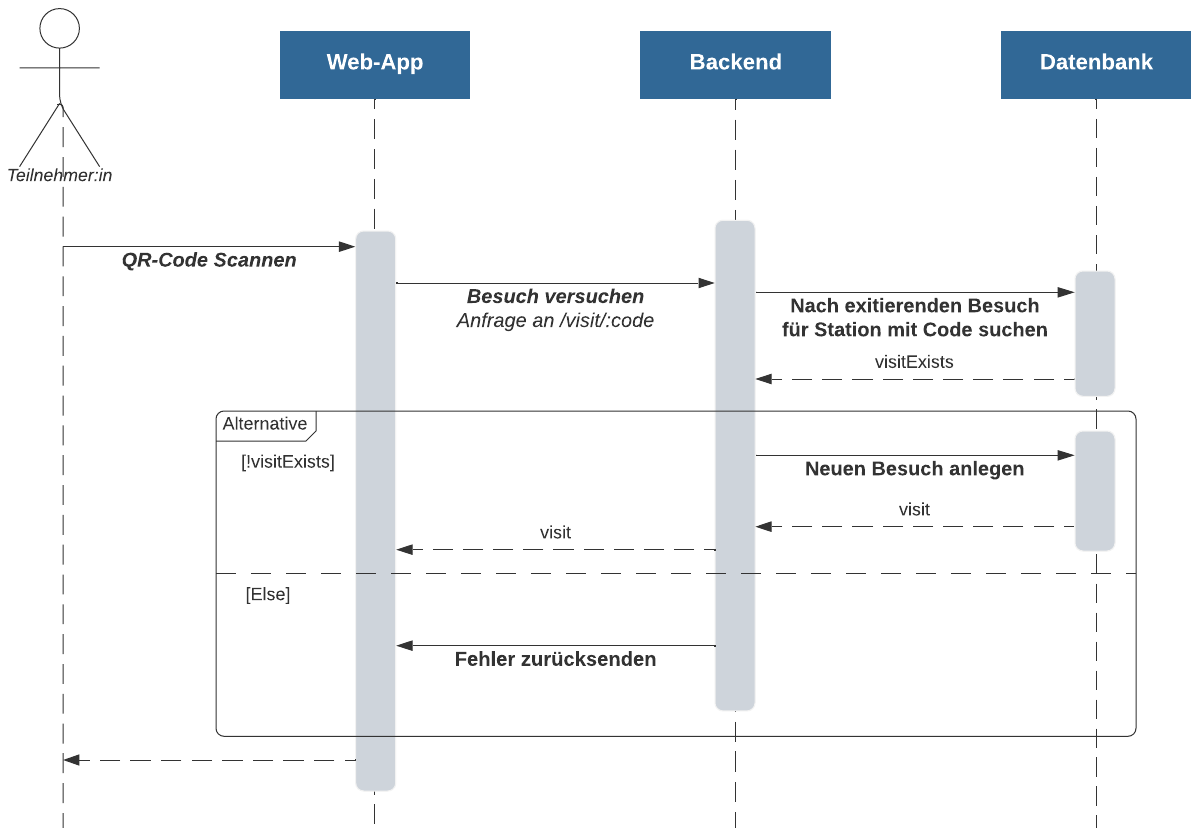
\includegraphics[width=\linewidth]{impl/sequence_visit.png}
    \caption{Interaktion eines Teilnehmenden mit der Visit API}
    \label{fig:impl-backend-visit-seq}
\end{figure}

Um eine Station zu besuchen, wird eine POST-Anfrage an \textit{/visit/:code}
abgeschickt, wobei \textit{:code} den Code der Station darstellt. Sollten
Teilnehmende die angegebene Station bereits besucht haben, wird ein
entsprechender Fehlercode zurückgegeben. Andernfalls werden die Daten des
Besuchs, inklusive der Stations-ID, zurückgegeben, um in der Web-App die
Weiterleitung zur entsprechenden Stationsseite zu ermöglichen. Die Datenstruktur
der Stationsbesuche ist in \autoref{fig:impl-backend-visit-data} zu sehen.

\begin{figure}[htpb]
    \centering
    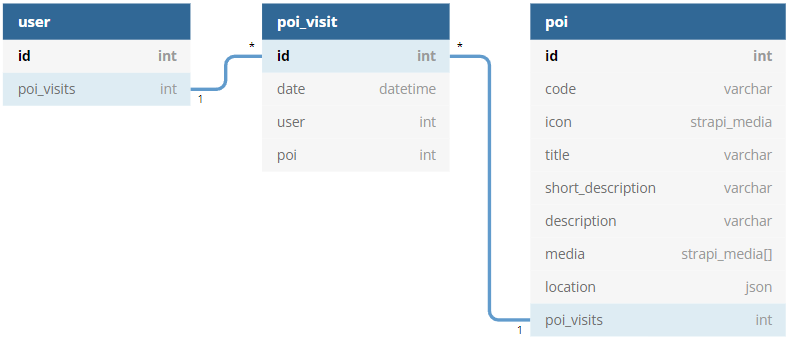
\includegraphics[width=\linewidth]{impl/uml_poi.png}
    \caption{Datenstruktur der Station in Verbindung mit Nutzenden. Intern werden Stationen als \textit{poi} (Point of Interest)
        bezeichnet.}
    \label{fig:impl-backend-visit-data}
\end{figure}

Die Stationsbesuche werden dabei bewusst in einer separaten Tabelle gespeichert,
um die Daten später einfacher filtern zu können und das Speichern des
Besuch-Zeitpunkts zu ermöglichen.

Das Abschließen von Abzeichen besitzt für Bild- und Textabzeichen einige
Parallelen zum Besuchen von Stationen. Auch hier gilt die Einschränkung, dass
ein bereits eingereichtes Abzeichen nicht erneut eingereicht werden können soll,
solange die Einreichung nicht abgelehnt wurde. Hierfür wurde ebenfalls eine
weitere API hinzugefügt: die \textit{Complete} API. Die Interaktion von
Teilnehmenden mit der Complete API ist in
\autoref{fig:impl-backend-complete-seq} grafisch aufbereitet.

\begin{figure}[ht]
    \centering
    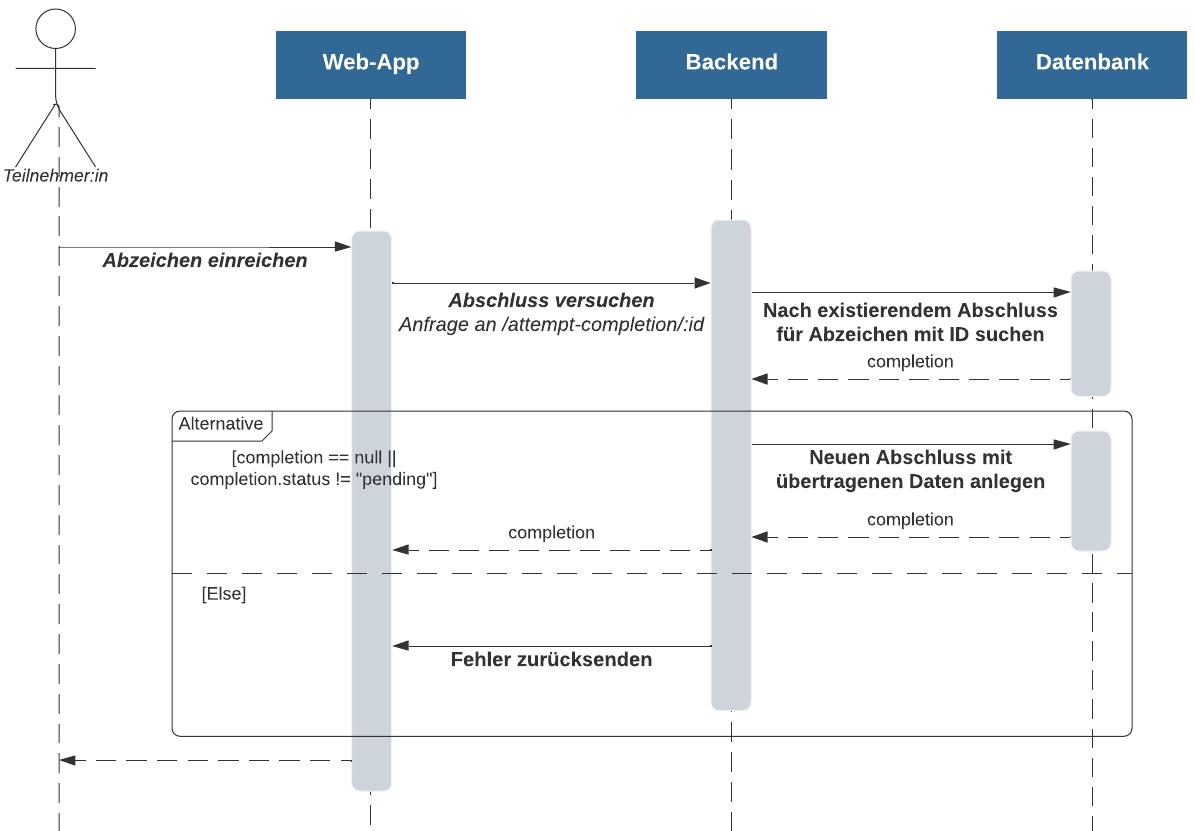
\includegraphics[width=\linewidth]{impl/sequence_completion.png}
    \caption{Interaktion eines Teilnehmenden mit der Complete API}
    \label{fig:impl-backend-complete-seq}
\end{figure}

Um ein Text- oder Bildabzeichen abzuschließen, wird eine POST-Anfrage an
\textit{/attempt-completion/:id} abgeschickt, wobei \textit{:id} die ID des
Abzeichens darstellt. Bei vorhandener ausstehender Abgabe wird ein Fehlercode
zurückgegeben. Andernfalls wird die übertragene Einreichung in der Datenbank des
Backends gespeichert. Im Gegensatz zur Visit API wird die Complete API auch von
Veranstaltenden genutzt, um Einreichungen zu bewerten. Über das in
\autoref{sec:impl-dashboard} beschriebene Dashboard können Veranstaltende die
Einreichung akzeptieren oder ablehnen. Daraufhin wird eine Anfrage an
\textit{/complete/:id} bzw. \textit{/dismiss/:id} gesendet, wobei die ID des
Abschlussversuchs übergeben wird (vgl.
\autoref{fig:impl-backend-complete-seq-v}). Wird ein Abschlussversuch gefunden,
wird sein Status entsprechend angepasst. Mögliche Statusangaben sind
\textit{pending}, \textit{denied} und \textit{accepted}. Der pending Status wird
dabei ausschließlich beim Erstellen des Versuchs verwendet. Diese Logik wird
jedoch nur für Text- oder Bildabzeichen genutzt. Für alle anderen Abzeichen wird
die entsprechende Bedingung im Code überprüft und bei erfüllter Bedingung direkt
ein Eintrag mit accepted für das jeweilige Abzeichen erstellt.

\begin{figure}[htpb]
    \centering
    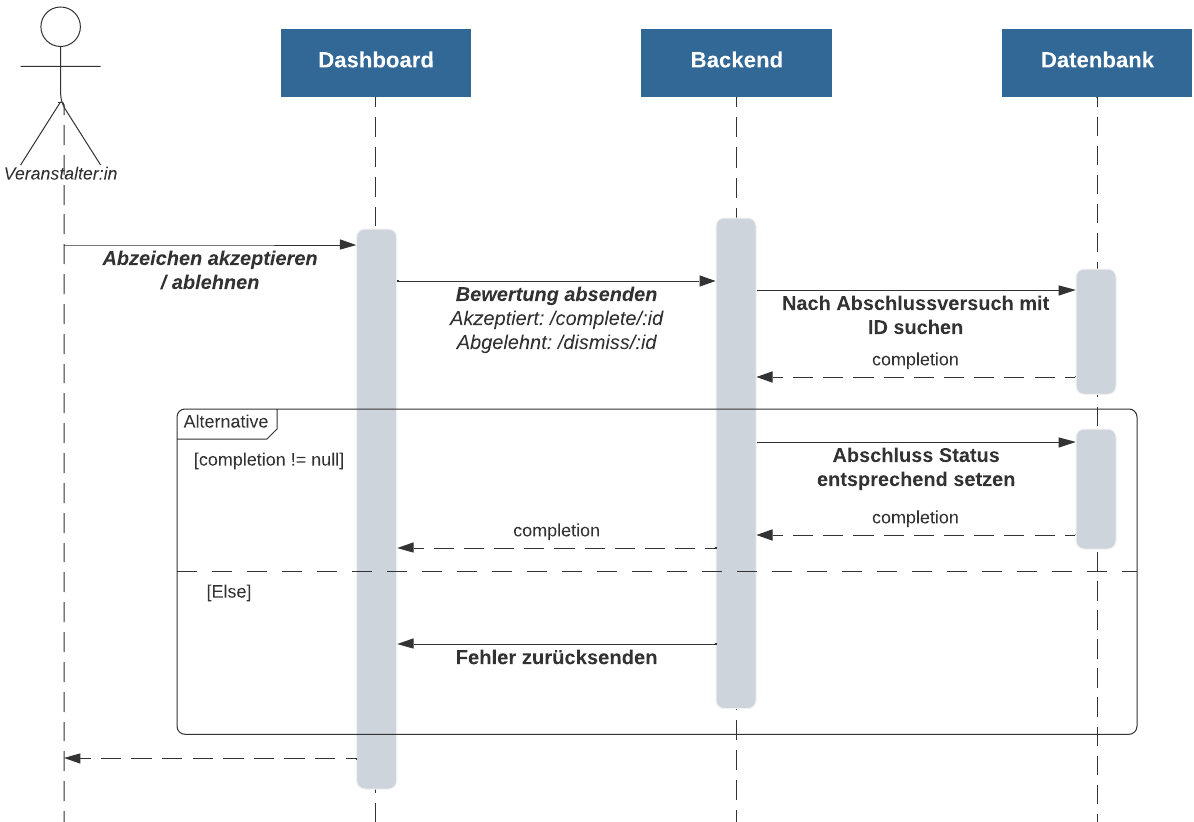
\includegraphics[width=\linewidth]{impl/sequence_completion_v.png}
    \caption{Interaktion eines Veranstaltenden mit der Complete API zum Bewerten einer Einreichung}
    \label{fig:impl-backend-complete-seq-v}
\end{figure}

Ähnlich zur Datenstruktur des Stationsbesuchs werden auch Abzeichen und ihre
dazugehörigen Abschlüsse auf zwei Tabellen aufgeteilt (\autoref{fig:impl-backend-completion-data}). Der Grund hierfür ist
ebenfalls die Erfassung der Erstellungs- und Bewertungszeit, sowie die einfache
Durchsuchung.

\begin{figure}[htpb]
    \centering
    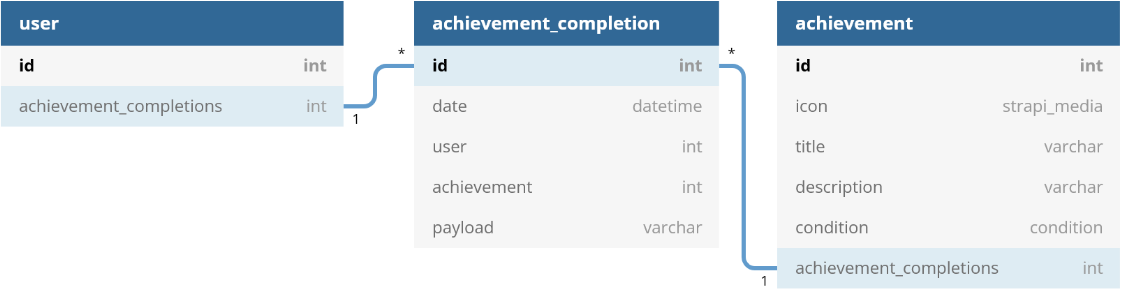
\includegraphics[width=\linewidth]{impl/uml_achievement.png}
    \caption{Datenstruktur der Abzeichen in Verbindung mit Nutzenden}
    \label{fig:impl-backend-completion-data}
\end{figure}

\newpage

Die Gruppen-Funktionalität erweitert Stationsbesuche und Abzeichen, indem
Besuche und Abschlüsse nicht mit Teilnehmenden, sondern analog mit deren Gruppe
verknüpft werden. Sobald ein Gruppenmitglied eine Station oder ein Abzeichen
abschließt, gilt dies somit für alle Mitglieder einer Gruppe. Da die
Gruppen-Funktionalität von Veranstaltenden optional oder ausgeschaltet werden
kann, muss es für Teilnehmende trotzdem möglich sein, diese Aktionen einzeln
auszuführen. Somit ergibt sich die in \autoref{fig:impl-backend-groups-data}
gezeigte Datenstruktur.

\begin{figure}[htpb]
    \centering
    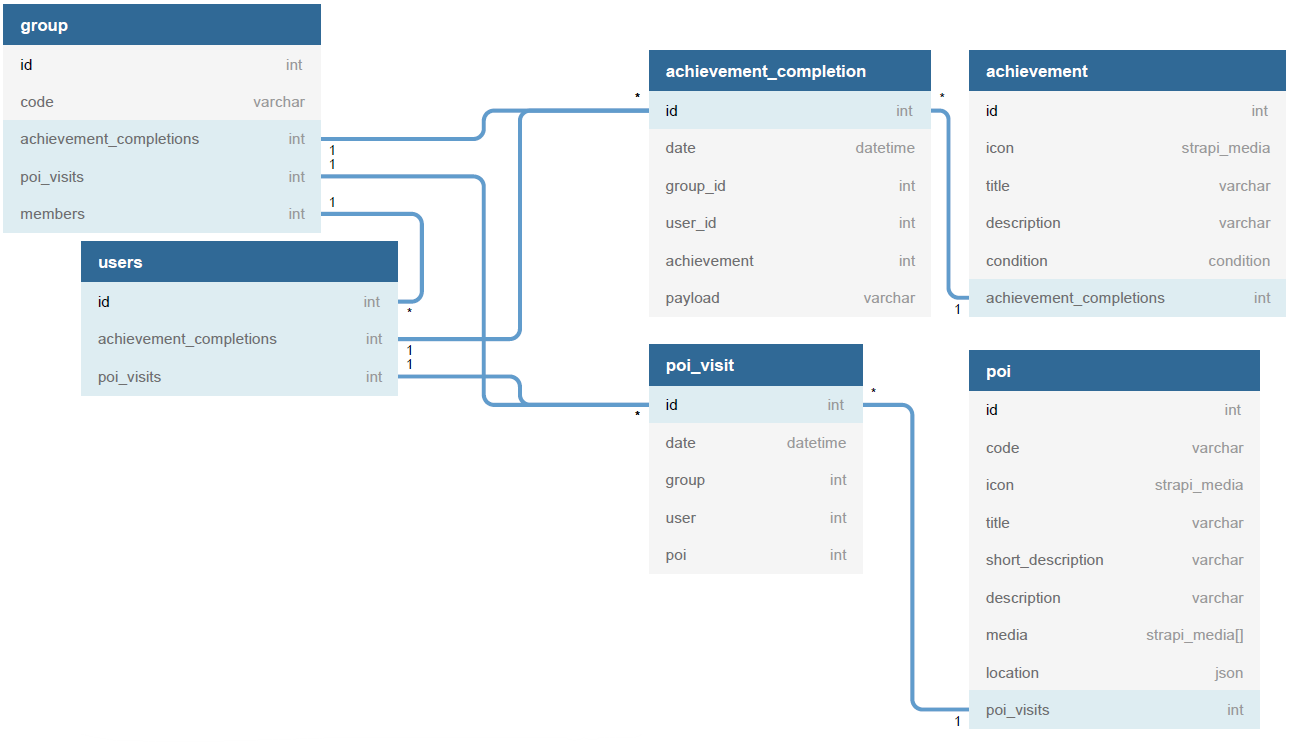
\includegraphics[width=\linewidth]{impl/uml_poi_achievement_group.png}
    \caption{Datenstruktur der Abzeichen und Stationen im Zusammenhang mit Gruppen}
    \label{fig:impl-backend-groups-data}
\end{figure}

Bevor Teilnehmende gemeinsam in einer Gruppe agieren können, müssen sie diese
erstellen oder ihr beitreten. Dies geschieht über eine POST-Anfrage an die
\textit{/groups/create} oder \textit{/groups/join} Route. Der
\textit{/groups/create} Route muss zusätzlich der Name der zu erstellenden
Gruppe übermittelt werden, während die \textit{/groups/join} Route den
Gruppen-Code der beitretenden Gruppe benötigt. Abschließend kann die Gruppe auch
wieder verlassen werden, indem eine POST-Anfrage an die \textit{/groups/leave}
Route geschickt wird.
\\
Sobald Teilnehmende Mitglied einer Gruppe sind, wird bei Stationsbesuchen und
Abzeicheneinreichungen oder -abschlüssen die Gruppe statt der Teilnehmenden
hinterlegt. Gleichzeitig wird beim Auslesen der Besuche und Abschlüsse nicht
mehr nach der Nutzer-ID, sondern der Gruppen-ID gefiltert. Alle
Gruppenmitglieder erhalten somit die neu erstellte Aktion. Eine Einschränkung
dieses Systems ist der temporäre Verlust von Daten bei Beitreten oder Verlassen
einer Gruppe, da jeweils nur Gruppen- bzw. Einzeldaten berücksichtigt werden.
Sobald Teilnehmende ihre Gruppe verlassen, werden wieder Einzeleinträge
angezeigt, da die Gruppeneinträge nicht mehr mit den Teilnehmenden
assoziiert sind. Dies gilt analog auch für das Beitreten einer Gruppe.

\subsection{Implementierung der Push-Benachrichtigungen} \label{ssec:impl-backend-push}

Gemäß \textit{Ft-V-5} (vgl. \ssecref{ssec:func-new}) sollen Teilnehmende von
Veranstaltenden jederzeit benachrichtigt werden können. Im Web-Kontext kann dies
über die Web-Push API erfolgen, welche es ermöglicht, auch außerhalb der Nutzung
der Web-App Benachrichtigungen zu erhalten. Jedoch wird die Web-Push API
von Safari auf iOS nicht unterstützt \cite{MDN2021}, weshalb eine Rückfalllösung
gebraucht wird. Unter Beachtung dieser Beschränkungen wurde ein drei-stufiges
Verfahren entwickelt, welches sich aus der Push API und einem Web-Socket Server
zusammensetzt. Im Folgenden werden diese beiden Technologien näher vorgestellt
und ihre Aufgabe und Interaktion im System präsentiert.

Der Web-Push Standard ermöglicht das Versenden und Empfangen von
Push-Benach\-richti\-gungen im Web-Kontext. Ein Endgerät, wie z. B. ein
Smartphone mit Browser, kann durch die Push API einen Push-Dienst abonnieren.
Durch das Abonnieren erhält das Endgerät eine eindeutige URL, welche von einem
Server, wie z. B. dem Backend, genutzt werden kann, um jederzeit Nachrichten an
das Endgerät zu senden. Ein besonderer Vorteil der Web-Push Standards ist das
Versenden von Nachrichten außerhalb der Browsernutzung. Sollten Teilnehmende die
Web-App zum Zeitpunkt des Versendens nicht ausführen, so wird die Nachricht
trotzdem empfangen. Die Funktionsweise der URL birgt jedoch ein
Sicherheitsrisiko, da jeder mit dieser URL beliebige Nachrichten an das
entsprechende Endgerät senden kann. Um diese Sicherheitslücke zu schließen, muss
jedes Abonnement verschlüsselt werden. Dies geschieht mit VAPID-Schlüsseln
\cite{VAPID}, wodurch auf dem Endgerät sichergestellt werden kann, das die
Nachricht vom richtigen Server stammt.

Web-Sockets hingegen sind für die Echtzeit-Kommunikation zwischen Endgerät und
Server gedacht. Sie ermöglichen das Senden und Empfangen von Nachrichten in
beide Richtungen. Somit kann das Endgerät, im Gegensatz zum Web-Push Standard,
auch Nachrichten an den Server schicken. Hierzu wird eine dauerhafte Verbindung
mit dem Server aufgebaut, welche jedoch mit dem Schließen der Web-App abbricht.
Im Vergleich zum Web-Push Standard eigenen sich Nachrichten über Web-Sockets
somit nur während der Nutzung der App. Jedoch werden für Web-Sockets keine
weiteren Verschlüsselungsmethoden, neben der Nutzung von HTTPS, benötigt. Zudem
vereinfachen JavaScript-Bibliotheken wie
Socket.IO\footnote{\url{https://socket.io/}}, welche in dieser Arbeit verwendet
wurde, die Nutzung von Web-Sockets und verwenden intern weitere Methoden, um
eine stabile Verbindung über eine breite Auswahl an Geräten zu garantieren
\cite{SocketIO2022}.


Basierend auf den Fähigkeiten der beiden vorgestellten Technologien wird ein
dreistufiges Verfahren zur Benachrichtigung entwickelt, welches durch
\autoref{fig:impl-backend-push} visualisiert wird. Wenn Veranstaltende eine
Nachricht versenden, wird zunächst das Versenden mit Web-Push versucht. Sollte
dies fehlschlagen, wird die Nachricht stattdessen über eine Web-Socket
Verbindung versendet. Falls auch dies fehlschlägt, wird die Nachricht im
Nutzerprofil gespeichert. Sobald Teilnehmende sich wieder mit dem Server
verbinden, wird dieser Vorgang erneut versucht. Allerdings wird die Nachricht in
diesem Fall verworfen, sollte die Nachricht weder per Web-Push noch Web-Sockets
versendet werden können (\autoref{fig:impl-backend-push-connect}).

\begin{figure}[htpb]
    \centering
    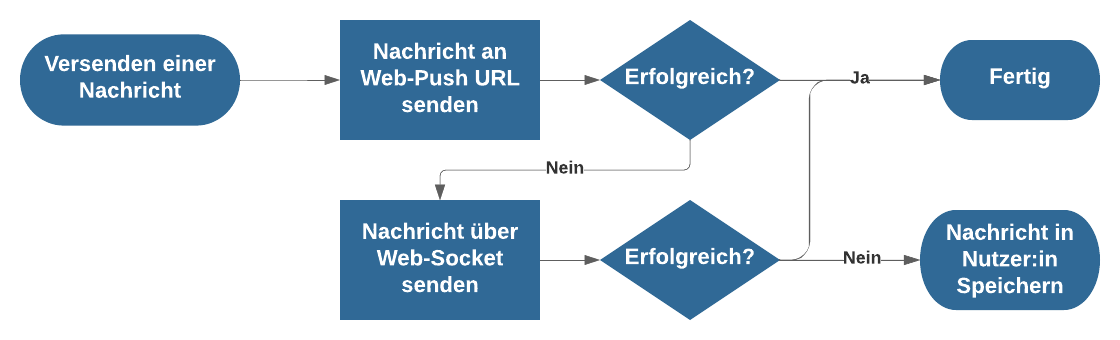
\includegraphics[width=\linewidth]{impl/flow_push.png}
    \caption{Verfahren zum Versenden von Benachrichtigungen an Teilnehmende}
    \label{fig:impl-backend-push}
\end{figure}

\begin{figure}[htpb]
    \centering
    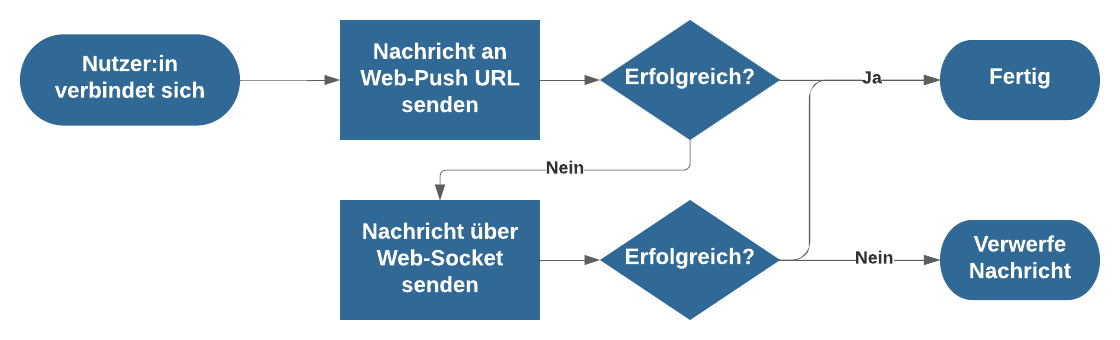
\includegraphics[width=\linewidth]{impl/flow_push_connect.png}
    \caption{Verfahren bei ausstehenden Benachrichtigungen}
    \label{fig:impl-backend-push-connect}
\end{figure}

\subsection{Implementierung der Feedback-Funktionalität}

Die Feedback-Funktionalität baut auf der Implementierung der
Push-Benachrichtigungen auf. Sobald Veranstaltende eine neue Feedback-Anfrage
verschicken, wird diese an alle Teilnehmende über das in
\ssecref{ssec:impl-backend-push} beschriebene Verfahren gesendet. Dabei wird
jede Feedback-Anfrage mit einer eindeutigen ID versehen, um die Antworten später
noch zur jeweiligen Anfrage zuordnen zu können. Die Datenstruktur des
Feedback-Systems wird in \autoref{fig:impl-backend-feedback-data} dargestellt.
Jede verschickte Feedback-Anfrage ist hierbei ein Eintrag in der
\textit{feedback} Tabelle, während die Antworten der Teilnehmenden als Einträge
in der \textit{feedback-response} Tabelle gespeichert werden. Hierzu wird die
Antwort als POST-Anfrage an \textit{/feedback/respond} gesendet.

\begin{figure}[htpb]
    \centering
    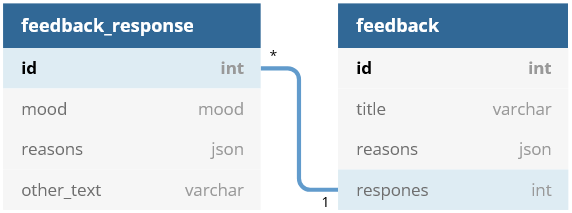
\includegraphics[width=0.6\linewidth]{impl/uml_feedback.png}
    \caption{Datenstruktur des Feedback-Systems}
    \label{fig:impl-backend-feedback-data}
\end{figure}

%\subsection{Softwarequalität}

% - Aussagekräftige Fehlermeldungen ->
% - Softwaretests

\section{Implementierung des Frontends}

Dieser Abschnitt präsentiert die bedeutendsten technischen Aspekte des
Frontends. Zunächst wird der Aufbau des Projekts und die Nutzung des Vue CLI
betrachtet. Daraufhin wird die Komponentenstruktur am Beispiel der interaktiven
Karte näher erläutert. Abschließend werden das native App-Erlebnis und die
Fortschrittsspeicherung aufgegriffen.

\subsection{Struktur mit Vue CLI} \label{ssec:impl-frontend-structure}

Zur Erstellung und Verwaltung des Projekts wurde das \textit{Vue
CLI}\footnote{\url{https://cli.vuejs.org/}} genutzt. Vue CLI ist ein
Kommandozeilenprogramm, welches die Einrichtung und Verwaltung von komplexeren
Vue Projekten stark vereinfacht. Das Erstellen eines Projekts erfolgt nach
Installation des Vue CLI durch den Befehl \lstinline[style=code, language=bash,
style=inline]{vue create <projekt-name>}. Während der Erstellung des Projekts
können zusätzliche Plugins ausgewählt werden, welche einige Vue-spezifische oder
allgemeine Funktionalitäten hinzufügen. Für dieses Projekt wurden die Plugins
aus \autoref{table:impl-frontend-vuecli-plugins} zur Installation ausgewählt.
Die Struktur des Vue-Projekts dieser Arbeit wird in
\autoref{fig:impl-frontend-vuecli-dir} präsentiert. Die fettgedruckten
Verzeichnisse sind nicht durch das Vue CLI generiert worden, sondern wurden
manuell erstellt. Nachfolgend wird die Struktur näher erläutert.

\begin{table}[htpb]
    \caption{Gewählte Vue CLI Plugins und ihre Funktion}
    \label{table:impl-frontend-vuecli-plugins}
    \begin{threeparttable}[t]
        \def\arraystretch{1.25}
        \centering
        \begin{tabularx}{\textwidth}{lX}
            \uzlhline%
            \uzlemph{Plugin}     & \uzlemph{Funktion}                                                      \\
            \uzlhline%
            \textbf{TypeScript}\tnote{1}  & Ermöglicht die Nutzung von TypeScript innerhalb
            eines Vue Projekts. TypeScript ergänzt JavaScript um eine Syntax für
            Datentypen, welche besser Vorschläge in Entwicklungsumgebungen
            ermöglicht und vorzeitig Fehler aufzeigen kann.                                                \\
            \textbf{PWA Support} &
            Generiert alle nötigen Dateien und Konfigurationen, welche für die
            Nutzung einer PWA benötigt werden. Zudem wird die Anpassung von PWAs an
            die eigenen Bedürfnisse vereinfacht.                                                           \\
            \textbf{Router}      &
            Fügt \textit{vue-router}\tnote{2}und seine benötigten Dateien zum Projekt hinzu.
            Vue-router ermöglicht das Anlegen von und Navigieren zu mehreren (Unter-)Seiten
            innerhalb der Web-App.                                                                         \\
            \textbf{Vuex}\tnote{3}        & Ergänzt das Projekt um einen zentralisierten
            Speicher, welcher das einfache Verwalten von globalen Zuständen
            ermöglicht. Dies umfasst Daten wie z. B. den Standort des Nutzers,
            welcher in mehreren Teilen der App benötigt wird.                                              \\
            \uzlhline
        \end{tabularx}
        \vspace{-0.75cm}
        \begin{tablenotes}
            \item [1] \url{https://www.typescriptlang.org/}
            \item [2] \url{https://router.vuejs.org/}
            \item [3] \url{https://vuex.vuejs.org/}
        \end{tablenotes}
    \end{threeparttable}
\end{table}


\begin{figure}[htpb]
    \centering
    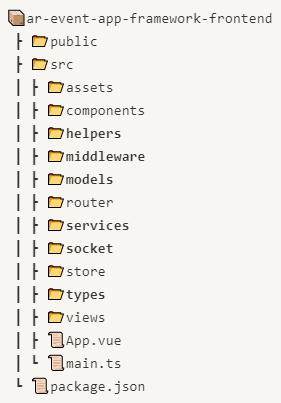
\includegraphics[width=0.45\linewidth]{impl/dir_frontend.png}
    \caption{Verzeichnisstruktur des Frontends mit Vue CLI}
    \label{fig:impl-frontend-vuecli-dir}
\end{figure}

Projekte, welche mit dem Vue CLI erstellt werden, gliedern sich im Wesentlichen
in zwei Ordner: \textit{public} und \textit{src}. Der \textit{public} Ordner
beinhaltet statische Datein, wie z. B. die \textit{index.html}, welche als
Template für die Vue-App genutzt wird. Weitere Dateien, die im \textit{public}
Ordner gefunden werden können, sind \textit{robots.txt}, welche
Suchmaschinen Hinweise zur Indexierung der Seite geben, und
\textit{favicon.ico}, welches vom Browser als Tab-Icon verwendet wird.

Der \textit{src} Ordner beinhaltet Code der eigentlichen Vue-App und ist in
weitere Ordner eingeteilt. Diese Ordner unterteilen den Code der App in seine
Aufgaben, wie z. B. das Anzeigen von Inhalten oder Abfragen von externen Daten.
Den Einstiegspunkt der App bilden hierbei die \textit{main.ts} und
\textit{App.vue}. In ihnen wird die Vue-App initialisiert und das grundlegende
Layout festgelegt. Plugins und globale Stylesheets werden hierbei in der
\textit{main.ts} eingebunden. Die \textit{App.vue} stellt hingegen die oberste
Vue-Kompontente dar, in welcher die gesamte Web-App dargestellt wird. Dauerhaft
sichtbare Elemente, wie die Navigationsleiste, wurden hier angelegt, um
duplizierten Code zu vermeiden.

Alle Ansichten befinden sich im \textit{views} Ordner. Die Ansichten selbst
nutzen meist mehrere Komponenten aus dem \textit{components} Ordner. Dies
ermöglicht das Wiederverwenden von Komponenten in mehreren Ansichten, wodurch
duplizierter Code vermieden werden kann. Zudem ermöglichen Komponenten das
Abkapseln bestimmter Logik, um die Vue-App klarer zu strukturieren. Bilder und
andere Dateien, welche fest in der App eingebunden werden, sind im
\textit{assets} Ordner zu finden.

Die einzelnen Ansichten lassen sich jeweils über ihre URL aufrufen. Hierzu wird
diese, sowie einige weitere Optionen, innerhalb der \textit{vue-router}
Konfiguration im \textit{router} Ordner festgelegt. Zudem beinhaltet der
\textit{store} Ordner den im vorherigen Abschnitt erwähnten globalen
\textit{Vuex} Speicher. Dieser wird genutzt, um Daten wie die Position der
Teilnehmenden oder Einstellungen abzuspeichern.

Alle bisher erwähnten Verzeichnisse und Dateien werden automatisch durch das Vue
CLI generiert. Zur besseren Übersichtlichkeit wurden weitere Ordner angelegt, um
eigene Funktionen nach Aufgaben zu gruppieren. Die \textit{models} und
\textit{services} Ordner beinhalten Funktionen zur Abfrage von Daten aus dem
Backend. Hierbei werden in \textit{models} die Typen der verschiedenen
Datenstrukturen des Backends repliziert. Die Anfrage-Funktionen des
\textit{services} Verzeichnisses nutzen diese Typen, um in der Vue-App die
Typisierung von externen Anfragen zu erlauben. Somit können Fehler in der
Nutzung der abgefragten Daten schneller erkannt werden. Der \textit{helpers}
Ordner enthält einige allgemeinere, hilfreiche Funktionen, welche in vielen
Teilen der Vue-App genutzt werden. Im \textit{middleware} Ordner sind sogenannte
\textit{Middlewares} zu finden. In diesem Kontext handelt es sich hierbei um
Funktionen, welche bei der Navigation zwischen Ansichten aufgerufen werden, um
z. B. zu kontrollieren, ob Teilnehmende authentifiziert sind. Das \textit{types}
Verzeichnis enthält TypeScript Typen für Pakete, welche keine Typen besitzen.
Somit können auch für diese Pakete die Vorteile von TypeScript genutzt werden.


\urldef\vuemixin\url{https://vuejs.org/guide/reusability/composables.html#comparisons-with-other-techniques}

Abschließend verfügt Vue.js seit der Version 3.0 über zwei verschiedene Arten,
den Aufbau von Komponenten organisieren: die Composition API und die Options
API. Die Options API ist hierbei die traditionelle Art Vue Komponenten zu
organisieren und war vor Version 3.0 die einzige Möglichkeit.
\autoref{fig:impl-frontend-vue-api-options} zeigt eine Beispiel-Komponente,
welche die Options API nutzt. Hierbei wird die Komponente nach der Art ihrer
Inhalte, der sogenannten \textit{Options}, strukturiert. Alle Methoden, Variablen und
übergebenen Werte werden jeweils gruppiert angegeben. Diese Art der
Strukturierung ermöglicht einen einheitlichen Aufbau über große Projekte. Jedoch
besitzt sie auch einige große Nachteile, wenn Teile der Komponente extrahiert
und wiederverwendbar gestaltet werden sollen\footnote{\vuemixin}.

\begin{figure}[htpb]
    \centering
    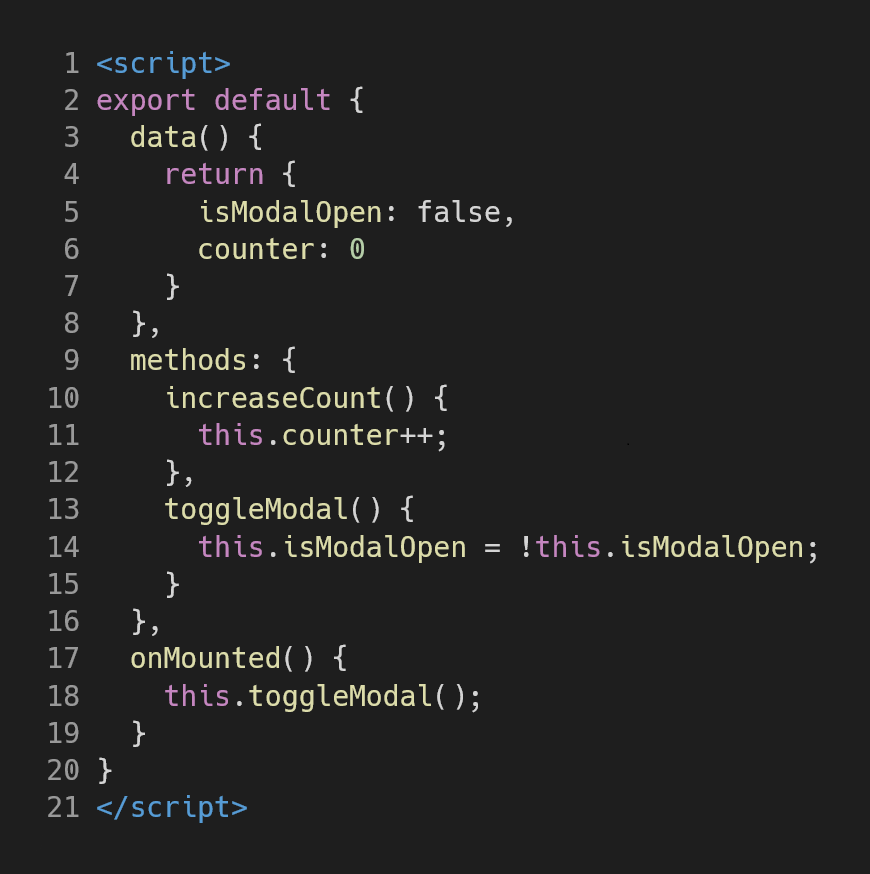
\includegraphics[width=0.65\linewidth]{impl/code_options.png}
    \caption{Beispiel-Komponente mit der Options API (Nur Script)}
    \label{fig:impl-frontend-vue-api-options}
\end{figure}

\urldef\vuecomp\url{https://vuejs.org/guide/extras/composition-api-faq.html#why-composition-api}
\urldef\vuets\url{https://vuejs.org/guide/extras/composition-api-faq.html#better-type-inference}

Die Composition API wurde konzipiert, um dieses und weitere Probleme zu beheben.
Anstatt Optionen anzugeben, werden die gewünschten Funktionalitäten importiert
und in beliebiger Struktur genutzt. Somit kann der Code nach seiner Funktion
gruppiert werden. Zum Vergleich ist die Composition API Version der
Beispiel-Komponente auf \autoref{fig:impl-frontend-vue-api-composition} zu
sehen. Zusätzlich wird TypeScript in der Composition API besser
unterstützt\footnote{\vuets}. In dieser Arbeit wird, aufgrund der vorgestellten
Vorteile und Empfehlung der offiziellen Dokumentation\footnote{\vuecomp}, die
Composition API genutzt.

\begin{figure}[htpb]
    \centering
    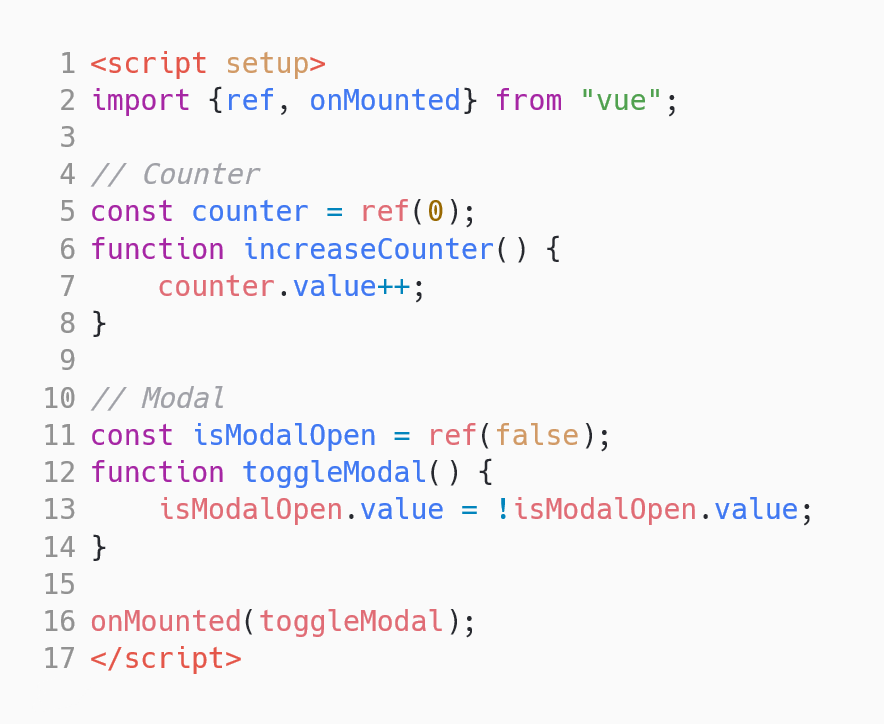
\includegraphics[width=0.65\linewidth]{impl/code_composition.png}
    \caption{Beispiel-Komponente mit der Composition API (Nur Script)}
    \label{fig:impl-frontend-vue-api-composition}
\end{figure}

%\subsection{API-Kommunikation}

\subsection{Komponentenstruktur}

Wie in \ssecref{ssec:impl-frontend-structure} beschrieben, besteht die Vue-App
aus einer Hierarchie an Ansichten und Komponenten. Im Folgenden wird am Beispiel
der interaktiven Karte aufgezeigt, wie diese Strukturen entwickelt wurden.
Hierfür wurde die Hierarchie der interaktiven Karte vereinfacht grafisch
dargestellt (\autoref{fig:impl-frontend-components-structure}).

\begin{figure}[htpb]
    \centering
    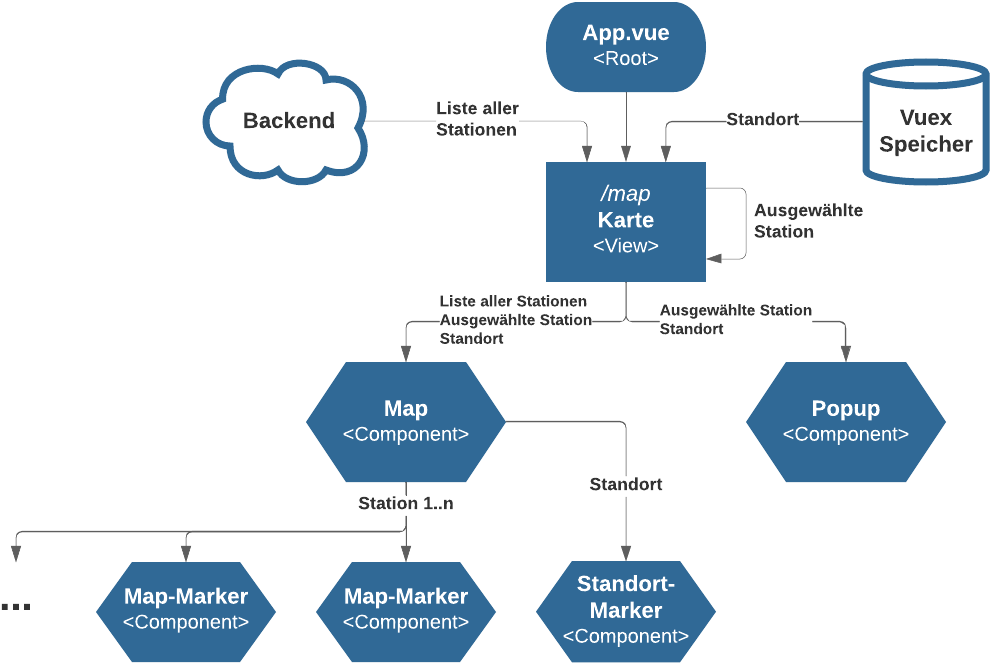
\includegraphics[width=\linewidth]{impl/component_map.png}
    \caption{Vereinfachter hierarchischer Aufbau der interaktiven Karte}
    \label{fig:impl-frontend-components-structure}
\end{figure}

Den Startpunkt der Hierarchie bildet, wie bereits in
\ssecref{ssec:impl-frontend-structure} beschrieben, die \textit{App.vue}. Im
Beispiel ist zurzeit die Karten-Ansicht ausgewählt, welche sich im
\textit{views} Verzeichnis befindet (\autoref{fig:impl-frontend-dirs} links,
\textit{Map.vue}). Diese wird durch ihren zugehörigen Pfad \textit{/map}
erreicht, welcher so im vue-router definiert wurde. Die Aufgabe der
Karten-Ansicht ist das Anzeigen aller Stationen, welche sie vom Backend anfragt.
Zusätzlich wird der Standort aus dem Vuex Speicher benötigt, welcher zur
Berechnung der Distanz und dem Anzeigen auf der Karte genutzt wird. Intern
überwacht die Karten-Ansicht zudem, welche Station aktuell ausgewählt ist.

\begin{figure}[htpb]
    \centering
    \begin{minipage}{.5\textwidth}
        \centering
        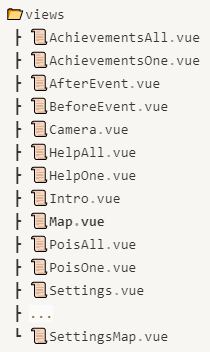
\includegraphics[width=.7\linewidth]{impl/dir_frontend_views.png}
    \end{minipage}%
    \begin{minipage}{.5\textwidth}
        \centering
        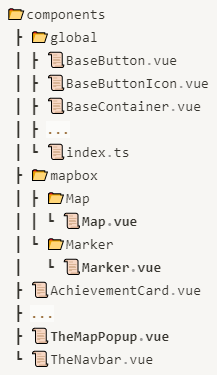
\includegraphics[width=.7\linewidth]{impl/dir_frontend_components.png}
    \end{minipage}
    \caption{Ausschnitt der Inhalte der \textit{views} und \textit{components}
    Verzeichnisse. Die Strukturierung und Benennung der Inhalte folgt dem Vue
    Style Guide \cite{You2022b}}
    \label{fig:impl-frontend-dirs}
\end{figure}

Diese Daten werden nach Bedarf an die Komponenten der Ansicht weitergegeben. Die
Karten-Ansicht besteht hierbei im Wesentlichen aus zwei Komponenten: der
interaktiven Karte (\textit{mapbox/Map/Map.vue}) und einem Pop-up
(\textit{TheMapPopup.vue}), welche sich im \textit{components} Verzeichnis
befinden (\autoref{fig:impl-frontend-dirs} rechts). Wie
\autoref{fig:impl-frontend-components-structure} zu entnehmen ist, erhält die
\textit{Map}-Komponente alle drei Daten der Karten-Ansicht, während das Pop-up
lediglich die ausgewählte Station und den Standort übergeben bekommt. Die
interaktive Karte ist hierbei nur für das Anzeigen der Karte, nicht aber der
Stationsicons, verantwortlich.

Um die Stationen anzuzeigen wird intern die Map-Marker Komponente genutzt. Für
jede in der Liste vorhandene Station wird eine Map-Marker Komponente
instanziiert und mit den Daten der jeweiligen Station versorgt. Hieraus werden
Icon und Position der Station entnommen, um diese korrekt anzuzeigen. Zudem
übernimmt die Map-Marker Komponente die Anpassung des Icons, falls die Station
ausgewählt ist oder bereits besucht wurde. Der Standort wiederum benötigt diese
Logik nicht und wird separat verwendet.

Die Pop-up Komponente nutzt die übergebene, ausgewählte Station, um ihre
Informationen wie Titel und Beschreibung anzuzeigen. Zusätzlich wird der
Standort verwendet, um die Distanz zur ausgewählten Station zu berechnen und
anzuzeigen. Intern setzen sich diese Komponenten noch aus weiteren Komponenten
zusammen, wie z. B. einer Icon-Komponente. Zur Übersichtlichkeit und
Verständlichkeit wurde dieses Beispiel jedoch vereinfacht.

Dieser hierarchische Aufbau und die Weitergabe der Daten an untergeordnete
Komponenten findet sich in der gesamten Vue-App wieder. Hierdurch können
Komponenten im System an vielen Stellen wiederverwendet werden, was
Entwicklungszeit spart und unterschiedliche Fehler in sich wiederholendem Code
vermeidet.

\subsection{Natives App-Erlebnis}
% Enkodierung des UI-Zustandes in der URL

Aufgrund der technischen Limitierungen ist eine native App im Rahmen dieser
Bachelorarbeit nicht möglich (vgl. \ssecref{ssec:analysis-old-tech}). Um
Teilnehmenden trotzdem ein möglichst natives App-Erlebnis zu ermöglichen, wurden
einige Maßnahmen eingesetzt. Nachfolgend wird erläutert wie der
\textit{vue-router} und die \textit{PWA}-Funktionalität hierfür genutzt wurden.

Traditionelle Webseiten müssen für jede aufgerufene Seite eine neue Anfrage an
den jeweiligen Server stellen. Dies ist meist mit einer längeren Wartezeit
verbunden. Jedoch werden bei Interaktionen mit einer Wartezeiten von mehr als
einer Sekunde bereits die Gedankengänge von Nutzenden unterbrochen und die
Interaktion fühlt sich wahrnehmbar verzögert an \cite{Nielsen1994b}. Um dieses
Problem zu umgehen, wird im Rahmen dieser Arbeit das \textit{vue-router} Paket
verwendet. Im Gegensatz zu traditioneller Navigation zwischen Seiten wird bei
der Verwendung von vue-router der Großteil der Navigation mithilfe von
JavaScript übernommen.

Anstatt bei jedem Aufruf erneut die HTML-Seite zu laden, wird nur noch eine
HTML-Seite angefragt, welche alle benötigten Daten der restlichen Anwendung
enthält. Bei jedem Seitenwechsel wird der Inhalt der Seite mithilfe des
JavaScript-Codes ausgetauscht. Dies verkürzt die Ladezeit und erlaubt es, die
Übergänge zwischen den Seiten nach Bedarf anzupassen. Das Prinzip dieser
gebündelten Seite nennt sich \textit{Singe-Page-Application (SPA)}.

Ein Nachteil von SPAs ist die Größe der Dateien beim ersten Aufruf. Um dieses
Problem zu minimieren, werden die Dateien meist stark komprimiert. Zudem lassen
sich verschiedene Teile der SPA nach Bedarf aufteilen und nachladen. Auch wenn
hier wieder eine Anfrage an den Server gestellt werden muss, ist dies schneller
als das Laden einer kompletten Seite. Zudem kann hier die PWA-Funktionalität
genutzt werden.

Progressive Web-Apps ermöglichen u. a. das Vorladen und Speichern von Webseiten,
um diese auch offline nutzen zu können. Hierzu werden JavaScript \textit{Service
Worker} genutzt. Service Worker sind JavaScript Prozesse, welche auf einem
separaten Thread ausgeführt werden und auch nach dem Schließen der Seite noch
aktiv sind. In ihnen können Dateien festgelegt werden, welche beim ersten Aufruf
der Seite direkt geladen und gespeichert werden sollen. Obwohl dies eine längere
Ladezeit zum ersten Aufruf bedeutet, werden alle weiteren Navigationen
zusätzlich beschleunigt, während die übertragenen Daten minimiert werden.
Besonders die Minimierung der übertragenen Daten spielt eine wichtige Rolle im
mobilen Kontext durch meist begrenztes Datenvolumen in Mobilfunkverträgen.

Zudem werden Service Worker benötigt, um Push-Benachrichtigungen zu empfangen.
Die Notifications
API\footnote{\url{https://developer.mozilla.org/en-US/docs/Web/API/Notifications_API}}
erlaubt es native Benachrichtigungen zu erstellen, welche das native
App-Erlebnis födern.

\subsection{Persistente Nutzerdatenspeicherung}

Da die Nutzung der App sich über mehrere Wochen erstrecken kann (vgl.
\autoref{sec:analysis-context}), ist die sichere Speicherung der Fortschritte
der Teilnehmenden ein wichtiger Faktor. Um dies zu gewährleisten werden die
Fortschrittsdaten auf dem Server in einem Nutzerprofil gespeichert. Dieses
Profil wird automatisch mit dem Akzeptieren der Datenschutzerklärung erstellt.
Da Teilnehmende keine identifizierenden Daten, wie z. B. eine E-Mail Adresse,
angeben müssen, wird stattdessen eine eindeutige ID generiert. Diese ID basiert
auf dem Browser Fingerprint der Teilnehmenden. Der Browser Fingerprint setzt
sich aus vielen auslesbaren Eigenschaften des Browsers zusammen. Hierzu gehören
z. B. die Bildschirmgröße, installierten Schriftarten, genutzte Hardware oder
Implementierungsunterschiede der verschiedenen
Browser\footnote{\url{https://fingerprintjs.com/blog/browser-fingerprinting-techniques/}}
(\autoref{fig:impl-frontend-browser-fingerprinting}). In dieser Arbeit wird
die JavaScript Bibliothek \textit{FinterprintJS} \cite{FingerprintJS2022}
genutzt, um die ID zu generieren.

\begin{figure}[htpb]
    \centering
    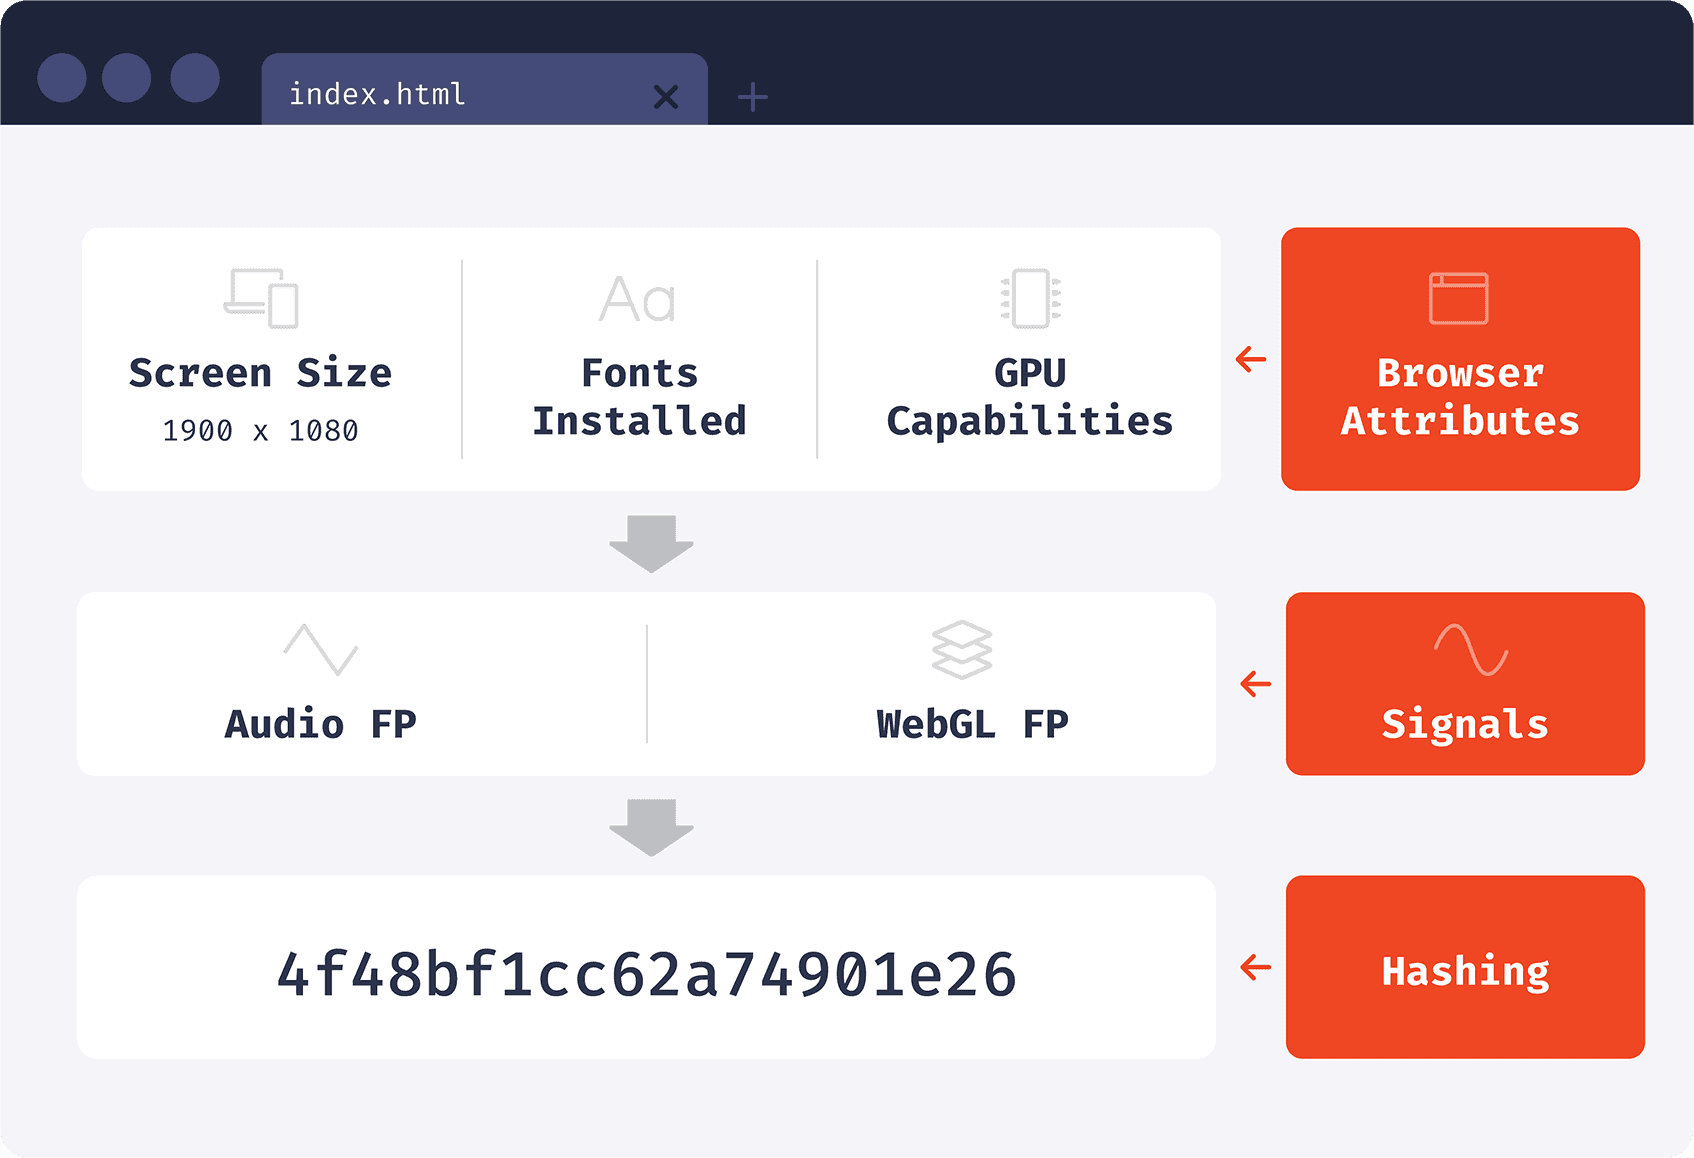
\includegraphics[width=.8\linewidth]{impl/browser_fingerprinting.png}
    \caption{Ausschnitt der genutzten Attribute zur Identifizierung des Browsers
    \cite{FingerprintJS2022}}
    \label{fig:impl-frontend-browser-fingerprinting}
\end{figure}

Nachdem die ID generiert wurde, wird sie als Nutzername und Passwort verwendet,
um einen neuen Account zu erstellen. Für alle weiteren Aktionen innerhalb der
Web-App, wie z. B. dem Besuchen von Stationen, wird der Account in der Anfrage
genutzt. Somit können die ausgeführten Aktionen im Nutzerprofil der
Teilnehmenden hinterlegt werden. Der Vorteil des Browser Fingerprinting liegt
hierbei in seiner Eigenschaft langlebig zu sein. Über mehrere Wochen kann
ein Browser Fingerprint für das gleiche Gerät unverändert bleiben. Somit ist die
Wahrscheinlichkeit hoch, dass selbst nach dem Löschen des Browserspeichers die
gleiche ID generiert wird. Folglich wird der gleiche Nutzeraccount verwendet und
ein Datenverlust vermieden.

\section{Implementierung des Dashboards} \label{sec:impl-dashboard}

In diesem Abschnitt wird die Implementierung des Dashboards erläutert. Da es
sich hierbei um ein Strapi Plugin handelt, wird zunächst der Aufbau eines
Plugins beschrieben. Daraufhin wird die Implementierung der visuellen
Aufbereitung der Daten erläutert. Abschließend wird das Location-Picker Plugin
implementiert, welches die Eingabe von Standortdaten vereinfacht.

\subsection{Aufbau eines Strapi Plugins}

Nachdem in \ssecref{ssec:impl-backend-structure} bereits die grundlegende
Struktur eines Strapi Projekts erklärt wurde, wird in diesem Abschnitt der
Aufbau eines Plugins innerhalb Strapis näher erläutert. In
\autoref{fig:impl-dashboard-dirs} wird die grundlegende Verzeichnisstruktur
eines Strapi Plugins präsentiert. Da jedes Plugin eine eigene API besitzt, ist
die Funktion der \textit{config, controllers} und \textit{services} Ordner
identisch zu den gleichnamigen Ordnern in \ssecref{ssec:impl-backend-structure}.
Das Dashboard Plugin besitzt keine eigene API, weshalb der Inhalt dieser Ordner
zu vernachlässigen ist. Der wesentliche Teil des Plugins, die
Benutzeroberfläche, befindet sich im \textit{admin} Ordner. Da Strapi für die
Entwicklung der Plugins React nutzt (vgl. \autoref{sec:frameworks}), stellt der
\textit{admin} Ordner das Stammverzeichnis einer React-Anwendung dar. Im
Folgenden werden die einzelnen Verzeichnisse und Dateien dieser Anwendung näher erläutert.

\begin{figure}[htpb]
    \centering
    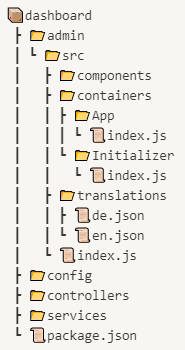
\includegraphics[width=.3\linewidth]{impl/dir_dashboard.png}
    \caption{Verzeichnisstruktur eines Strapi Plugins, stark vereinfacht}
    \label{fig:impl-dashboard-dirs}
\end{figure}

Die \textit{src/index.js} dient zur Konfiguration und Einbindung des Plugins in
die Strapi Oberfläche. In ihr wird u. a. Name, Icon, Beschreibung, die
Verlinkung in der Oberfläche und benötigte Berechtigungen zum Aufrufen des
Plugins eingestellt. Anschließend bestehen zwei Möglichkeiten das Plugin in
Strapi einzubinden: als Oberfläche / API oder als Bearbeitungsfeld. Das
Dashboard selbst wird hierbei als ersteres eingebunden. Auf die Einbindung und
Entwicklung eines Bearbeitungsfeldes wird in
\ssecref{ssec:impl-dashboard-location-plugin} eingegangen.

Der Kern der React-Anwendung befindet sich im \textit{sec/containers}
Verzeichnis. Dort werden die eigentlichen React-Komponenten implementiert. In
\autoref{fig:impl-dashboard-dirs} werden zwei besondere Komponenten
hervorgehoben: die \textit{App} und \textit{Initializer} Komponenten. Die
Initializer Komponente kann verwendet werden, um eigene Logik vor Plugin-Start
auszuführen. Die App Komponente bildet hingegen die Haupt-Komponente der
Anwendung, welche beim Aufrufen des Dashboards angezeigt wird. In ihr werden die
verschiedenen Ansichten des Dashboards mit URLs verknüpft. Neben App und
Initializer existieren noch viele weitere, zur Übersichtlichkeit ausgeblendete,
React-Komponenten, welche die einzelnen Ansichten des Dashboards beinhalten.
Unterkomponenten, welche in verschiedenen Ansichten wiederholt benutzt werden,
befinden sich im \textit{src/components} Verzeichnis.

Schließlich können im \textit{src/translations} Ordner Übersetzungen der
benutzten Texte angelegt werden. Hierbei gibt es für jede Sprache eine
entsprechend benannte Datei (z. B. \textit{de.json}), in welcher Texte unter IDs
abgespeichert werden können (\autoref{fig:impl-dashboard-translation}). Diese
IDs werden anschließend in den Komponenten benutzt, um je nach eingestellter
Sprache der Nutzenden, die Texte der entsprechenden Sprache zu nutzen.

\begin{figure}[htpb]
    \centering
    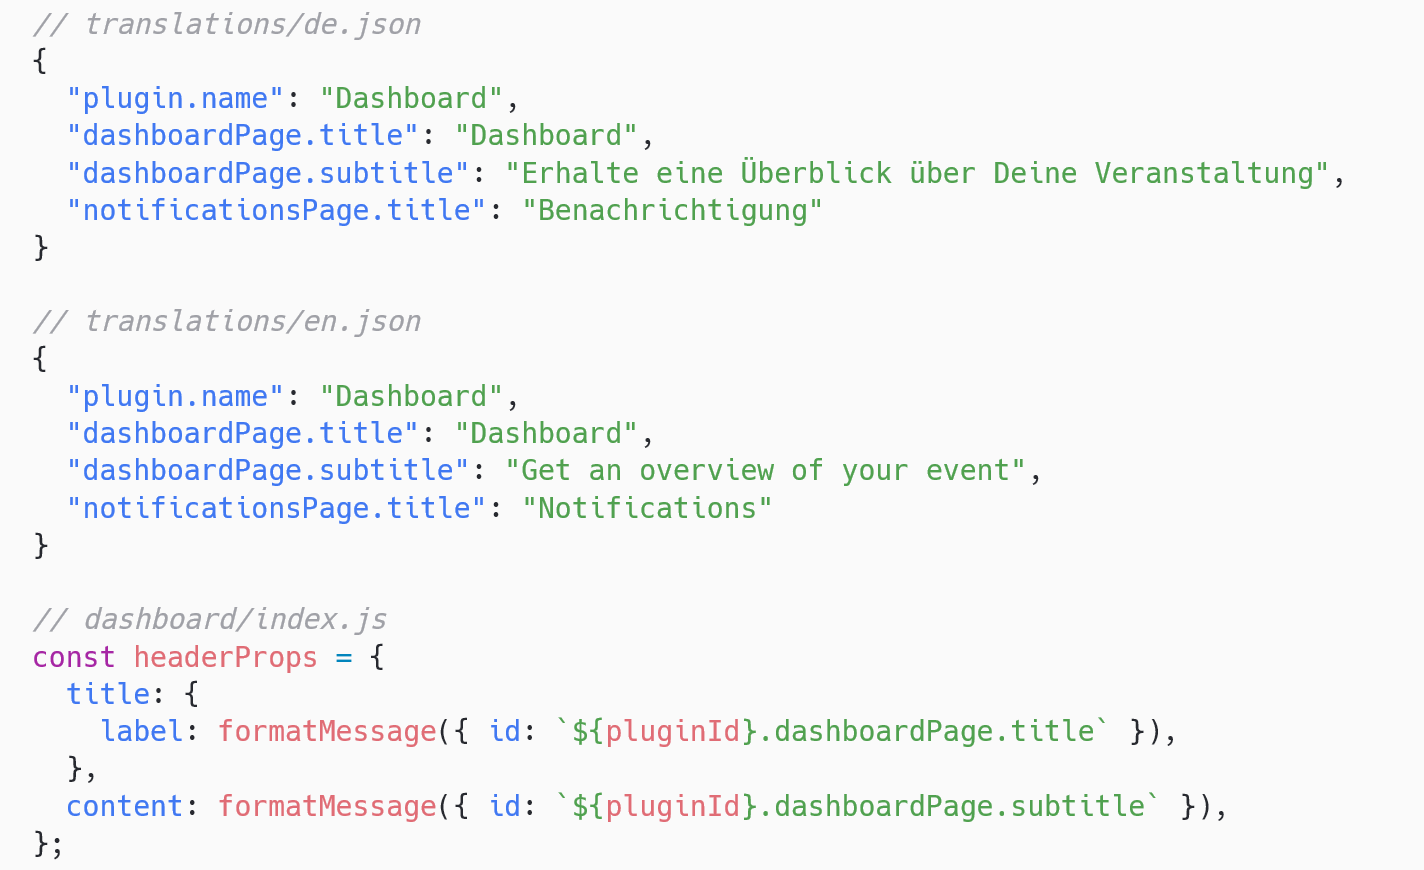
\includegraphics[width=\linewidth]{impl/dasboard_translation.png}
    \caption{Aufbau und Verwendung der Übersetzungen}
    \label{fig:impl-dashboard-translation}
\end{figure}

\subsection{Implementierung der Statistiken}

Eine der Hauptfunktionen des Dashboards ist das Überblicken der Veranstaltung
und seiner gesammelten Daten. Um dies zu ermöglichen wurden die Daten der
Teilnehmenden, Stationen, Abzeichen und Feedback-Anfragen im Dashboard visuell
aufbereitet. Nachfolgend wird erklärt wie diese Statistiken realisiert wurden.

Für die Darstellung der Statistiken wurde das Paket
\textit{victory}\footnote{\url{https://formidable.com/open-source/victory/}}
genutzt, welches speziell für React entwickelt wurde. \textit{Victory}
ermöglicht das einfache Erstellen von einer Vielzahl von Diagrammtypen, u. a.
auch Flächendiagrammen, welche zur Darstellung benutzt werden sollen (vgl.
\ssecref{ssec:interface-v}). Das Paket stellt hierfür einige Komponenten bereit,
mit welchen die Diagramme modular erstellt werden können (\autoref{fig:impl-dashboard-diagramm-code}).

\begin{figure}[htpb]
    \centering
    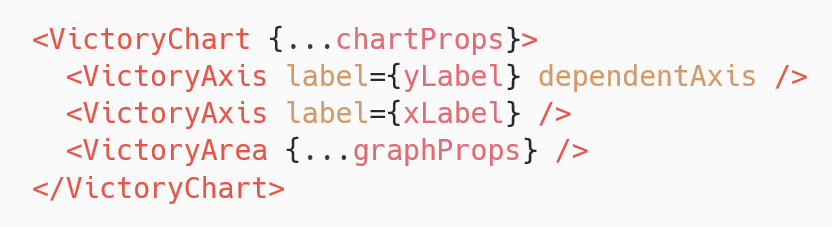
\includegraphics[width=0.7\linewidth]{impl/code_diagramms.png}
    \caption{Verwendung der Victory Komponenten}
    \label{fig:impl-dashboard-diagramm-code}
\end{figure}

Die für die Diagramme benötigten Daten werden von der \textit{Statistics API}
des Backends angefragt, welche vor dem Bereitstellen der Daten diese bereits
nach angegeben Merkmalen gruppiert oder sortiert. Im Fall der Statistiken zu
Besuchenden, Stationen und Abzeichen wird beispielsweise nach Datum der Aktion
sortiert, um diese korrekt im Diagramm wiederzugeben.

\subsection{Implementierung des Location-Picker Plugins} \label{ssec:impl-dashboard-location-plugin}

Der Standort einer Station ist eine fundamentalen Informationen. Jedoch besitzt
Strapi keine vorhandene Oberfläche oder Datentyp, um Standortdaten einzutragen.
Um die mühsame Eintragung von Längengrad und Breitengrad zu vermeiden, wurde ein
Plugin implementiert, welches das Setzen eines Standorts mithilfe einer
interaktiven Karte ermöglicht. Hierfür wurde die Strapi \textit{Field API}
genutzt, um das Location-Picker Plugin als Bearbeitungsfeld nutzen zu können
(\autoref{fig:impl-dashboard-location-code}). Im Gegensatz zum Dashboard Plugin
benötigt das Location-Picker Plugin keine Ansichten im \textit{src/containers}
Verzeichnis, da eine Komponente aus dem \textit{src/components} Verzeichnis
direkt importiert und genutzt wird. Die registrierte Komponente funktioniert
anschließend ähnlich wie die internen Datentypen von Strapi (vgl.
\ssecref{ssec:impl-backend-structure}). Jedoch kann sie nicht in Strapis
Oberfläche ausgewählt werden, sondern muss manuell in der entsprechenden
\textit{models/<model>.settings.json} eingetragen werden.

\begin{figure}[htpb]
    \centering
    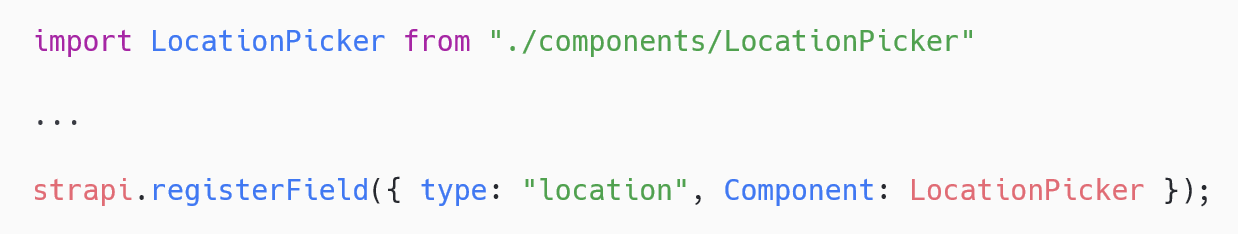
\includegraphics[width=0.9\linewidth]{impl/code_field_api.png}
    \caption{Registrierung einer Komponente als Strapi Feld}
    \label{fig:impl-dashboard-location-code}
\end{figure}

Des Weiteren bindet das Location-Picker Plugin eine Einstellungsansicht ein.
Diese wird mit den vorhandenen Einstellungen von Strapi zusammen angezeigt (\autoref{fig:impl-dashboard-location-settings}) und erlaubt es das Mapbox API
Access Token zusetzen. Jenes wird benötigt, da zur Implementierung der Karte das
Paket \textit{mapbox-gl} verwendet wird.

\begin{figure}[htpb]
    \centering
    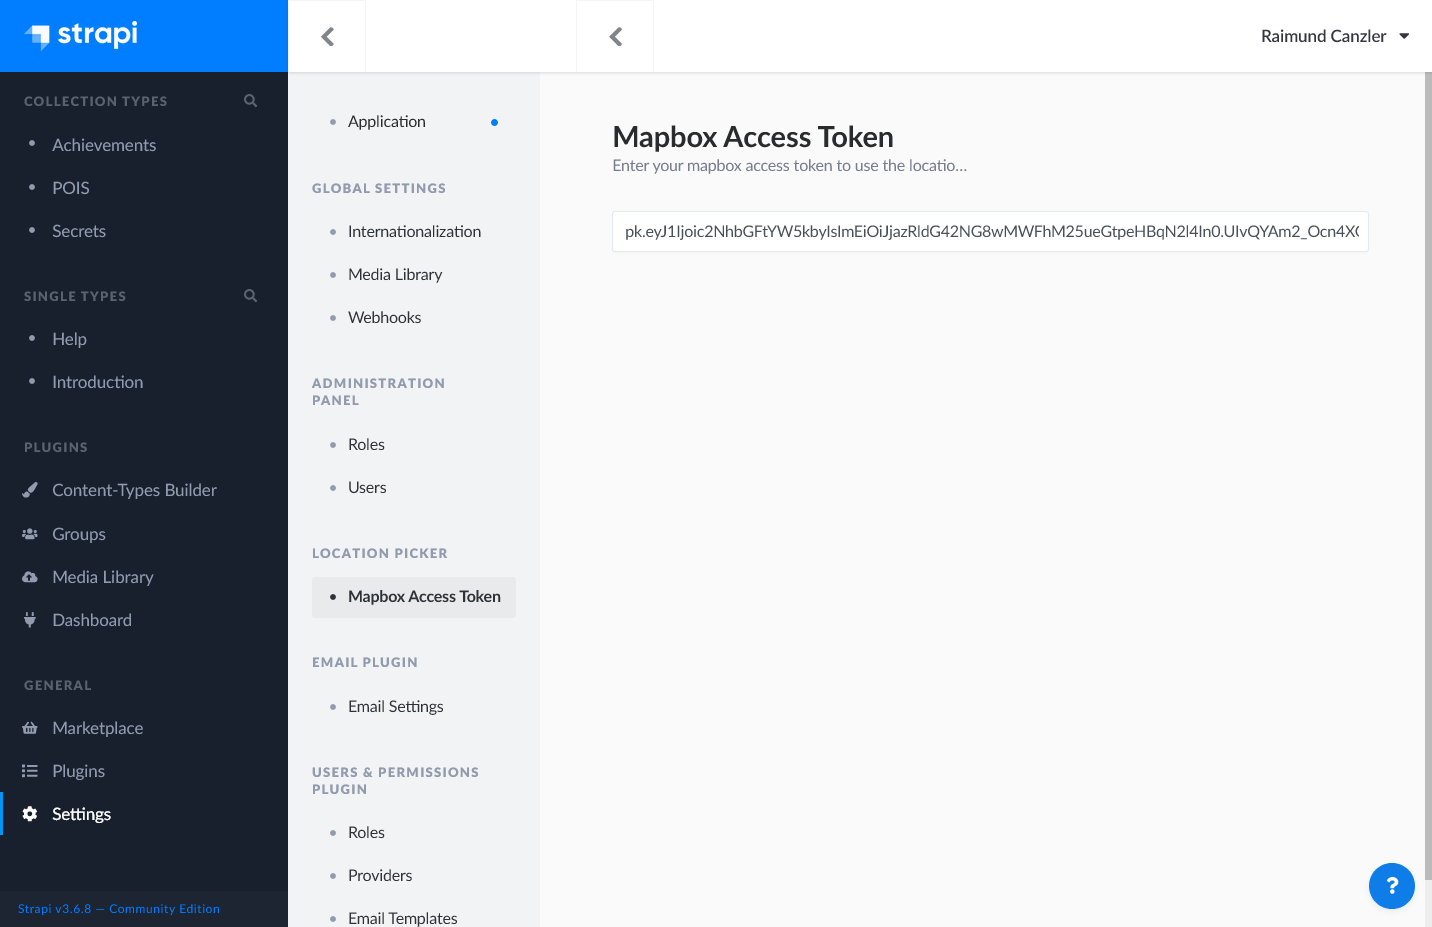
\includegraphics[width=\linewidth]{impl/settings_location_picker.png}
    \caption{Einstellungen des Mapbox API Access Tokens}
    \label{fig:impl-dashboard-location-settings}
\end{figure}


\section{Nutzung des Systems}

In diesem Abschnitt werden die nötigen Schritte aufgeführt, um das System in
Betrieb zu nehmen. Zuerst wird die Installation erklärt, gefolgt von der
Konfiguration und Ausführung des Systems. Aufgrund der Unterschiede zwischen
Web-App und Strapi, wird die Ausführung für beide Teile des Systems separat
beschrieben.

\subsection{Installation}

Um das System nutzen zu können, wird eine funktionierende Installation von
\textit{Node.js}\footnote{\url{https://nodejs.org/en/}} (Version 12.x.x oder
neuer) und des beigelieferten Paket-Managers
\textit{npm}\footnote{\url{https://www.npmjs.com/}} benötigt. Zudem wird die
Installation des Paket-Managers \textit{yarn} (\lstinline[style=code,
language=bash, style=inline]{npm install -g yarn}) empfohlen, da dieser zur
Entwicklung des Systems genutzt wurde. Anschließend sollte in beiden
Stammverzeichnissen des Systems (Web-App und Strapi) der Befehl
\lstinline[style=code, language=bash, style=inline]{yarn install} ausgeführt
werden.

\subsection{Konfiguration}

Bevor das System ausgeführt werden kann, müssen zwingend einige Einstellungen an
die jeweilige Umgebung angepasst werden. Hierzu existiert in beiden Projekten
eine \textit{.env} Datei. Diese beinhaltet für das System wichtige
Einstellungsmöglichkeiten, wie z. B. die URL der App oder den zu nutzenden Port
des Systems. Die Inhalte der beiden \textit{.env} Dateien sind in
\autoref{fig:impl-use-env} dargestellt.

\begin{figure}[htpb]
    \centering
    \begin{minipage}{.55\textwidth}
        \centering
        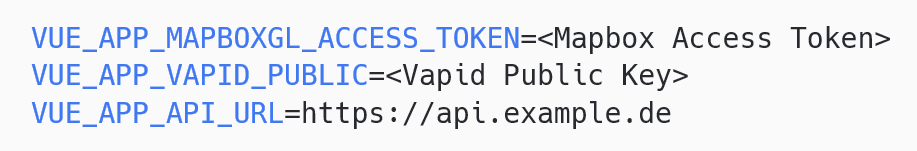
\includegraphics[width=.98\linewidth]{impl/env_frontend.png}
    \end{minipage}%
    \begin{minipage}{.45\textwidth}
        \centering
        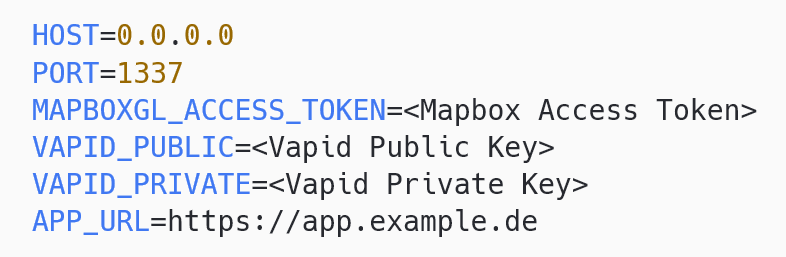
\includegraphics[width=.98\linewidth]{impl/env_backend.png}
    \end{minipage}
    \caption{Inhalte der \textit{.env} Datei im Frontend (links) und Backend (rechts)}
    \label{fig:impl-use-env}
\end{figure}

Hierbei ist vor allem der Mapbox API Access Token von hoher Bedeutung, da ohne
diesen die interaktiven Karten des Systems nicht funktionieren. Um ein Access
Token zu generieren, wird ein Mapbox Account vorausgesetzt. Die VAPID Keys
werden genutzt, um Push-Benachrichtigungen zu versenden (vgl.
\ssecref{ssec:impl-backend-push}). Um ein Paar an VAPId-Keys zu generieren, kann

\lstinline[style=code, language=bash, style=inline]{npx web-push generate-vapid-keys --json}

genutzt werden.

\subsection{Ausführung der Web-App}

% - Bauen der Vue-App
% - Auf Webserver packen, z. B. Nginx oder Netlify.

Zum Ausführen bzw. Bereitstellen der Web-App muss diese vorher noch „gebaut“
werden. Hierbei handelt es sich um einen Prozess, in dem der Quellcode auf ein
Minimum reduziert wird. Externe Pakete werden eingebunden und ungenutzter Code,
soweit möglich, entfernt. Um diesen Prozess anzustoßen, muss im
Stammverzeichnis der Web-App der Befehl \lstinline[style=code, language=bash, style=inline]{yarn build} ausgeführt werden. Nachdem der Bau-Prozess erfolgreich
abgeschlossen ist, sollte ein neues \textit{dist} Verzeichnis generiert wurden
sein. Dieses Verzeichnis kann nun zum statischen Hosting verwendet werden.

\subsection{Ausführung von Strapi}

Das Ausführen des Strapi Servers kann auf verschiedene Arten geschehen. Die
einfachste Methode bildet hierbei das direkte Starten des Servers. Dafür muss im
Stammverzeichnis des Strapi-Backends der Befehl \lstinline[style=code, language=bash, style=inline]{yarn start} aufgerufen werden. Hiermit wird der
Strapi Server in einem Modus gestartet, der keine Veränderungen der
Datenstruktur mehr erlaubt.

Alternativ kann die freie Containervirtualisierungs-Software
\textit{Docker}\footnote{\url{https://www.docker.com/}} genutzt werden. Diese
erlaubt es, den Strapi Server vom Rest des ausführenden Systems zu entkoppeln
und eine reproduzierbare Ausführungsumgebung zu schaffen. Für diese Methode wird
eine funktionierende Installation von Docker vorausgesetzt. Um ein neues
Docker-Image zu bauen, kann der Befehl

\lstinline[style=code,language=bash, style=inline]{docker build -t <name>/<tag> .}

im Stammverzeichnis des Strapi Servers ausgeführt werden. Dieser nutzt den dort
vorhandenen \textit{Dockerfile}, um ein neues Docker-Image zu erstellen.
Anschließend kann der \textit{docker-compose} Dienst genutzt werden, um das
Backend zusammen mit einer passenden Datenbank zu starten. Eine mögliche
Konfiguration wird dafür in \autoref{fig:impl-dashboard-docker} dargestellt.

\begin{figure}[htpb]
    \centering
    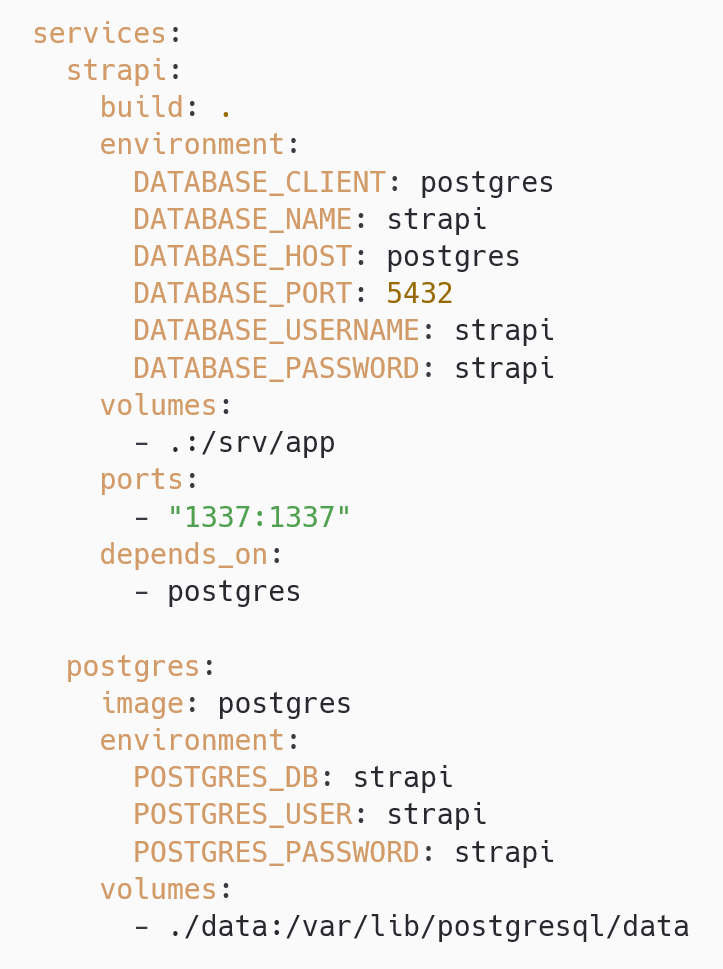
\includegraphics[width=0.5\linewidth]{impl/docker_compose.png}
    \caption{Docker Compose Konfiguration, welche das Backend zusammen mit einer PostgeSQL Datenbank startet und verbindet}
    \label{fig:impl-dashboard-docker}
\end{figure}